\documentclass[a4paper, 11pt, oneside]{article} 

\usepackage[utf8]{inputenc} % Required for inputting international characters
\usepackage[T1]{fontenc} % Output font encoding for international characters

% Custom titling format

\usepackage{secdot}
\usepackage{titling}
\usepackage[margin=1.5in]{geometry}
\date{\today}

% Allows bold and italics math

\usepackage{bm}


% Remove numbering from sections but keep them in TOC

\makeatletter
\def\@seccntformat#1{%
  \expandafter\ifx\csname c@#1\endcsname\c@section\else
  \csname the#1\endcsname\quad
  \fi}
\makeatother

\usepackage{amssymb}
\usepackage{amsmath}
\usepackage{graphicx}
\usepackage{animate}
\usepackage{floatrow}
\usepackage{caption}
\usepackage{booktabs}

\usepackage{svg}
\usepackage{siunitx}
\usepackage{tikz} % To generate the plot from csv
\usepackage{pgfplots}

% Allows to place the legend below plot

\pgfplotsset{compat=newest} 

% Allows to enter the units nicely

\usepgfplotslibrary{units} 


% Cute boxes

\usepackage{xcolor}
\usepackage[framemethod=default]{mdframed}

\newmdenv[skipabove=7pt,
          skipbelow=7pt,
          rightline=false,
          leftline=true,
          topline=false,
          bottomline=false,
          linecolor=orange!60!gray,
          backgroundcolor=gray!15,
          innerleftmargin=5pt,
          innerrightmargin=2pt,
          innertopmargin=5pt,
          leftmargin=0cm,
          rightmargin=0cm,
          linewidth=3pt,
          innerbottommargin=5pt]{cBox}
          
          
          
% Setting for writing code
      
\usepackage{minted}
\usepackage{algorithm}
\usepackage{algorithmic}
\usepackage{beramono}

\newenvironment{code}[2][]
 {\VerbatimEnvironment
  \begin{minted}[
        frame=lines,
        framesep=2mm,
        baselinestretch=1.2,
        bgcolor=bg,
        linenos,
        fontsize=\footnotesize
        ]{#2}}
 {\end{minted}}

% Defines background colour of code
\definecolor{bg}{rgb}{0.95, 0.95, 0.95}
 
% Adds the º symbol
\usepackage{gensymb}
 
 
% Includes "References" in the table of contents

\usepackage[nottoc]{tocbibind}

\usepackage[autostyle = true]{csquotes}

\usepackage[backend=biber,style=ieee]{biblatex}
\urlstyle{same}
\addbibresource{bibliography.bib}

% Allows subsubsubsections
 
\makeatletter
\renewcommand{\paragraph}{\@startsection{paragraph}{4}{0ex}%
    {-3.25ex plus -1ex minus -0.2ex}%
    {1.5ex plus 0.2ex}%
    {\normalfont\normalsize\bfseries}}
\makeatother
 
\stepcounter{secnumdepth}
\stepcounter{tocdepth}
 
% Hyperlinks settings

\usepackage{hyperref}

\hypersetup{
    colorlinks=false,
    linkcolor=blue,
    filecolor=magenta,      
    urlcolor=cyan,
}


% Settings of minted (Writing code)

\newenvironment{code}[2][]
 {\VerbatimEnvironment
  \begin{minted}[
        frame=lines,
        framesep=2mm,
        baselinestretch=1.2,
        bgcolor=bg,
        linenos,
        fontsize=\footnotesize]{#2}}
 {\end{minted}}
 

\newcommand{\inputcode}[2][vhdl]{\inputminted[frame=lines,
                                              framesep=2mm,
                                              baselinestretch=1.2,
                                              bgcolor=bg,
                                              linenos,
                                              fontsize=\footnotesize
                                              ]{#1}{#2}}



% Custom part page

% \usepackage{tikz} -> Included before
\usetikzlibrary{calc}

\makeatletter
\@addtoreset{section}{part}
\makeatother  

\renewcommand{\thepart}{\arabic{part}}
\def\topleft{4}

\newcommand{\cpart}[1]{
    \clearpage
    \stepcounter{part}
    \pagestyle{empty}
    \begin{tikzpicture}[overlay,remember picture]
    \coordinate(ptopleft) at ($(current page.north west)+(\topleft,0)$);
    \foreach \i in{0,.1,.2,.3,.5,.6,.9,1.1,1.2,1.3,1.5,1.6,1.8,1.9,2}
    \draw[gray!70]($(ptopleft)+(\i,0)$)--+(0,-\paperheight);
    \node[white,fill=black,minimum size=1.5cm](A) at ($(ptopleft)+(1,-2)$){\huge\thepart};
    \node [anchor=south,ultra thick,yshift=-1mm]at(A.north){\Large PART};
    \node [fill=white,anchor=north,very thick,right=-2mm,inner sep=5mm]at($(ptopleft)+(0,-0.5\paperheight)$){\Huge #1};
    \end{tikzpicture}
    \addcontentsline{toc}{part}{\thepart\hspace{1em}#1}
    \clearpage
    \pagestyle{plain}
}


%%---------------------------------------------------------------------------------------------
%% Document
%%---------------------------------------------------------------------------------------------

\begin{document} 

% ANIMATION ON = 1 / ANIMATION OFF = 0
\newcounter{ANIMATION}
\setcounter{ANIMATION}{1}

% Includes the title page
\begin{titlepage} % Suppresses headers and footers on the title page

    \fontfamily{stix}\selectfont
	\centering % Centre everything on the title page
	\scshape % Use small caps for all text on the title page
	\vspace*{\baselineskip} % White space at the top of the page
	
%------------------------------------------------------------------------------------------------
%	                                    Title
%------------------------------------------------------------------------------------------------
	\vspace{3\baselineskip}
	
	\rule{\textwidth}{1.6pt}\vspace*{-\baselineskip}\vspace*{2pt} % Thick horizontal rule
	\rule{\textwidth}{0.4pt} % Thin horizontal rule
	
	\vspace{0.75\baselineskip} % Whitespace above the title
	
	{\LARGE Digital Electronics\\ Project 2:\\Safe with combination lock\\} % Title
	
	\vspace{0.75\baselineskip} % Whitespace below the title
	
	\rule{\textwidth}{0.4pt}\vspace*{-\baselineskip}\vspace{3.2pt} % Thin horizontal rule
	\rule{\textwidth}{1.6pt} % Thick horizontal rule
	
	\vspace{1.5\baselineskip} % Whitespace after the title block


	%------------------------------------------------
	%	Editor(s)
	%------------------------------------------------
	
	{\scshape\Large Alejandro López Rodríguez \\ Ana Mª Casanova López \\ Raúl Gómez Fetes \\} % Editor list
	
	\vspace{1.5\baselineskip} % Whitespace below the editor list
	
	\textit{Universidad Politécnica de Valencia\\ ETSID\\} 
	
	\vspace{2\baselineskip} % Whitespace after the title block
	\thedate
	
	\vfill % Whitespace between editor names and publisher logo

\end{titlepage}

% Preface
\section*{Preface}
\thispagestyle{empty}
\setcounter{page}{0}

This project is the result of weeks of collaborative work between the authors. Designing, discussing and testing the different modules that conform it has helped us to better understand the course as well as to develop crucial key skills such as communication, teamwork, problem solving and time management. \medskip 

Before diving into the document there are some remarks that must be made to better understand the assignment:

\begin{itemize}
    \item Most of the GALs that we have used in this project use Finite State Machines to perform their different duties. In almost of all them, a synchronous reset is used in lieu of an asynchronous one. The decision was intentional since most of the FSMs end in a final steady state that waits for the reset signal to restart themselves. Besides, the clock frequency is very fast for a GAL, so it is almost impossible for them to miss the reset signal. We have tested this extensively and found no problem whatsoever in the execution of the code.
    
    \item All of the images, tables, and figures are vectorial, so feel free to zoom in if something is not big enough.
    
    \item There are hyperlinks in most of the pages that will take you to the specific section in which the mentioned topic is explained in more detail. We recommend that you use a PDF Viewer such as Adobe Acrobat or similar.
    
    \item We have also added hyperlinks to the references that we have used to elaborate the assignment. The full references list can be found at the end of the document.
    
    \item The project files can be found \textbf{\href{https://drive.google.com/drive/folders/1CNiwcC9CncEdfxiFuib3KTSMWgVY08vC?usp=sharing}{here}}. We strongly suggest having the Proteus file open alongside the PDF.
    
    \item In the Proteus file you will find instructions on how to operate the system.
\end{itemize}

\medskip

We sincerely hope you like the project. Please, feel free to comment on how you would improve certain aspects if you find it necessary. We are aware of the extension of the document and would like to apologize beforehand.\bigskip 

Finally, let us end this project and also this subject by saying that it has truly been a great pleasure having you as a teacher. We hope that somehow our paths cross again in the future. 


\clearpage

% Table of contents
\thispagestyle{empty}
\setcounter{page}{0}
\tableofcontents
\clearpage

% Add later

% \listoffigures
% \listoftables
% \clearpage

% Document


\section{Introduction}

A security box or safe-deposit box stores our personal belongings safely, only being accessible by ourselves or the ones we trust. It is common to have one at home, but they can also be found at hotel rooms. This device is usually a metal box, often with a concrete layer for not only making it more secure, but heavier, so that burglars have it more difficult to take it with them. The door mechanism is usually a multi-point lock, and the opening method depends on the security box. Different opening mechanisms are widely used in commercial security boxes, namely a key, a multi-combination mechanism, a keypad, a fingerprint scanner, and so on.

\subsection{Objectives}

The goal of this project is to develop the whole electronics part of a security box. The security box will be operated by a keypad in order to enter a 4-digit password. To set the password that the user wants, dip switches will be installed inside, so that only the user can change it.

\subsection{Opening sequence}
\label{sec:OPENING_SEQ}

To enter a password, the “start button” or asterisk \emph{*} must be pressed first. Then, the password can be introduced, with two restrictions:

\begin{itemize}
    \item Password must be a 4 digit number.
    \item Password must not have two or more consecutive repeated digits, i.e. $1122$, $1111$ or $1223$ are not valid.
\end{itemize}

\vspace{-0.2cm}

\medskip

In order to open/close the security box, the “enter password” button or hash \textit{\#}  must be pressed. Only then the password will be processed by the system. Once pressed, the password will appear on the screen for a brief amount of time.\medskip

After this, both passwords, the one entered by the keypad and the one stored inside the security box will be compared. If they are equal, after a few seconds an \textit{Open} message will appear, and, at the same time, a green LED will be switched on, which in real life would be the motor to open the multi-point lock; otherwise a message of \textit{Error} will be displayed and a red LED will be switched on, indicating that the passwords did not match.

\subsection{Password setting mechanism}

Once the security box is opened, the user has the option to set a new password. The mechanism involves 4 dip switches, one for each of the 4 digits.\medskip

Each digit must be in the range of 0 to 9 and must be introduced in binary, as each selector consists of four independent switches, being the top one the Most Significant Bit (MSB).\medskip

The new password must meet the requirements from Subsection \ref{sec:OPENING_SEQ}, because otherwise, the GALs will not be able to compare both passwords correctly.



\section{Implementation}
\subsection{Keypad}
\label{sec:KEYPAD}

The most common method of introducing the password of a security box is the keypad. This is due to its ease of use, and its low cost, compared for instance with a dial combination, or a fingerprint scanner.
\medskip

\begin{figure}[H]
    \centering
    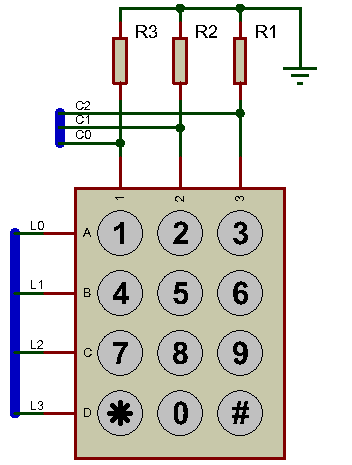
\includegraphics[scale = 0.8]{Graphics/KEYPAD/KEYPAD.PDF}
    \caption{Keypad from Proteus' Libraries}
    \label{fig:KEYPAD}
\end{figure}


In order to implement a keypad in our system, a HIGH level is introduced in one of the line rows and it is constantly circulated among them. When a button is pressed, depending on the column in which a HIGH level is detected and the position of the ‘1’ in the rows, the GAL will be able to show in the output the Binary Coded Decimal (BCD) representation of the number that has been pressed following this fashion:

\begin{table}[H]
    \centering
        \begin{tabular}[t]{lcccc}
            \toprule
            &\textbf{L3..L0}&\textbf{C2...C0}&\textbf{Button}&\textbf{BCD code}\\
            \midrule
                &    0001   & 001     & 1      & 0001     \\
                &    0010   & 001     & 4      & 0100     \\
                &    0100   & 001     & 7      & 0111     \\
                &    1000   & 001     & *      & 1100     \\
                &    0001   & 010     & 2      & 0010     \\
                &    0010   & 010     & 5      & 0101     \\
                &    0100   & 010     & 8      & 1000     \\
                &    1000   & 010     & 0      & 0000     \\
                &    0001   & 100     & 3      & 0011     \\
                &    0010   & 100     & 6      & 0110     \\
                &    0100   & 100     & 9      & 1001     \\
                &    1000   & 100     & \#     & 1111     \\
            \bottomrule
        \end{tabular}
        \caption{Reading to Button Conversion table ~\autocite{SLIDES_5}}
        \label{table: KEYPAD_TABLE}
\end{table}


A ring counter is used in order to rotate the HIGH input bit for the lines. It is a type of counter composed of flip-flops connected together to form a shift register, with the output of the last flip-flop fed to the input of the first, making a "circular" or "ring" structure. In this case, the ring must be initialized with a ‘1’ and after that, the bit will be rotating indefinitely. An example of such counter can be found attached below:

\begin{figure}[H]
    \centering
    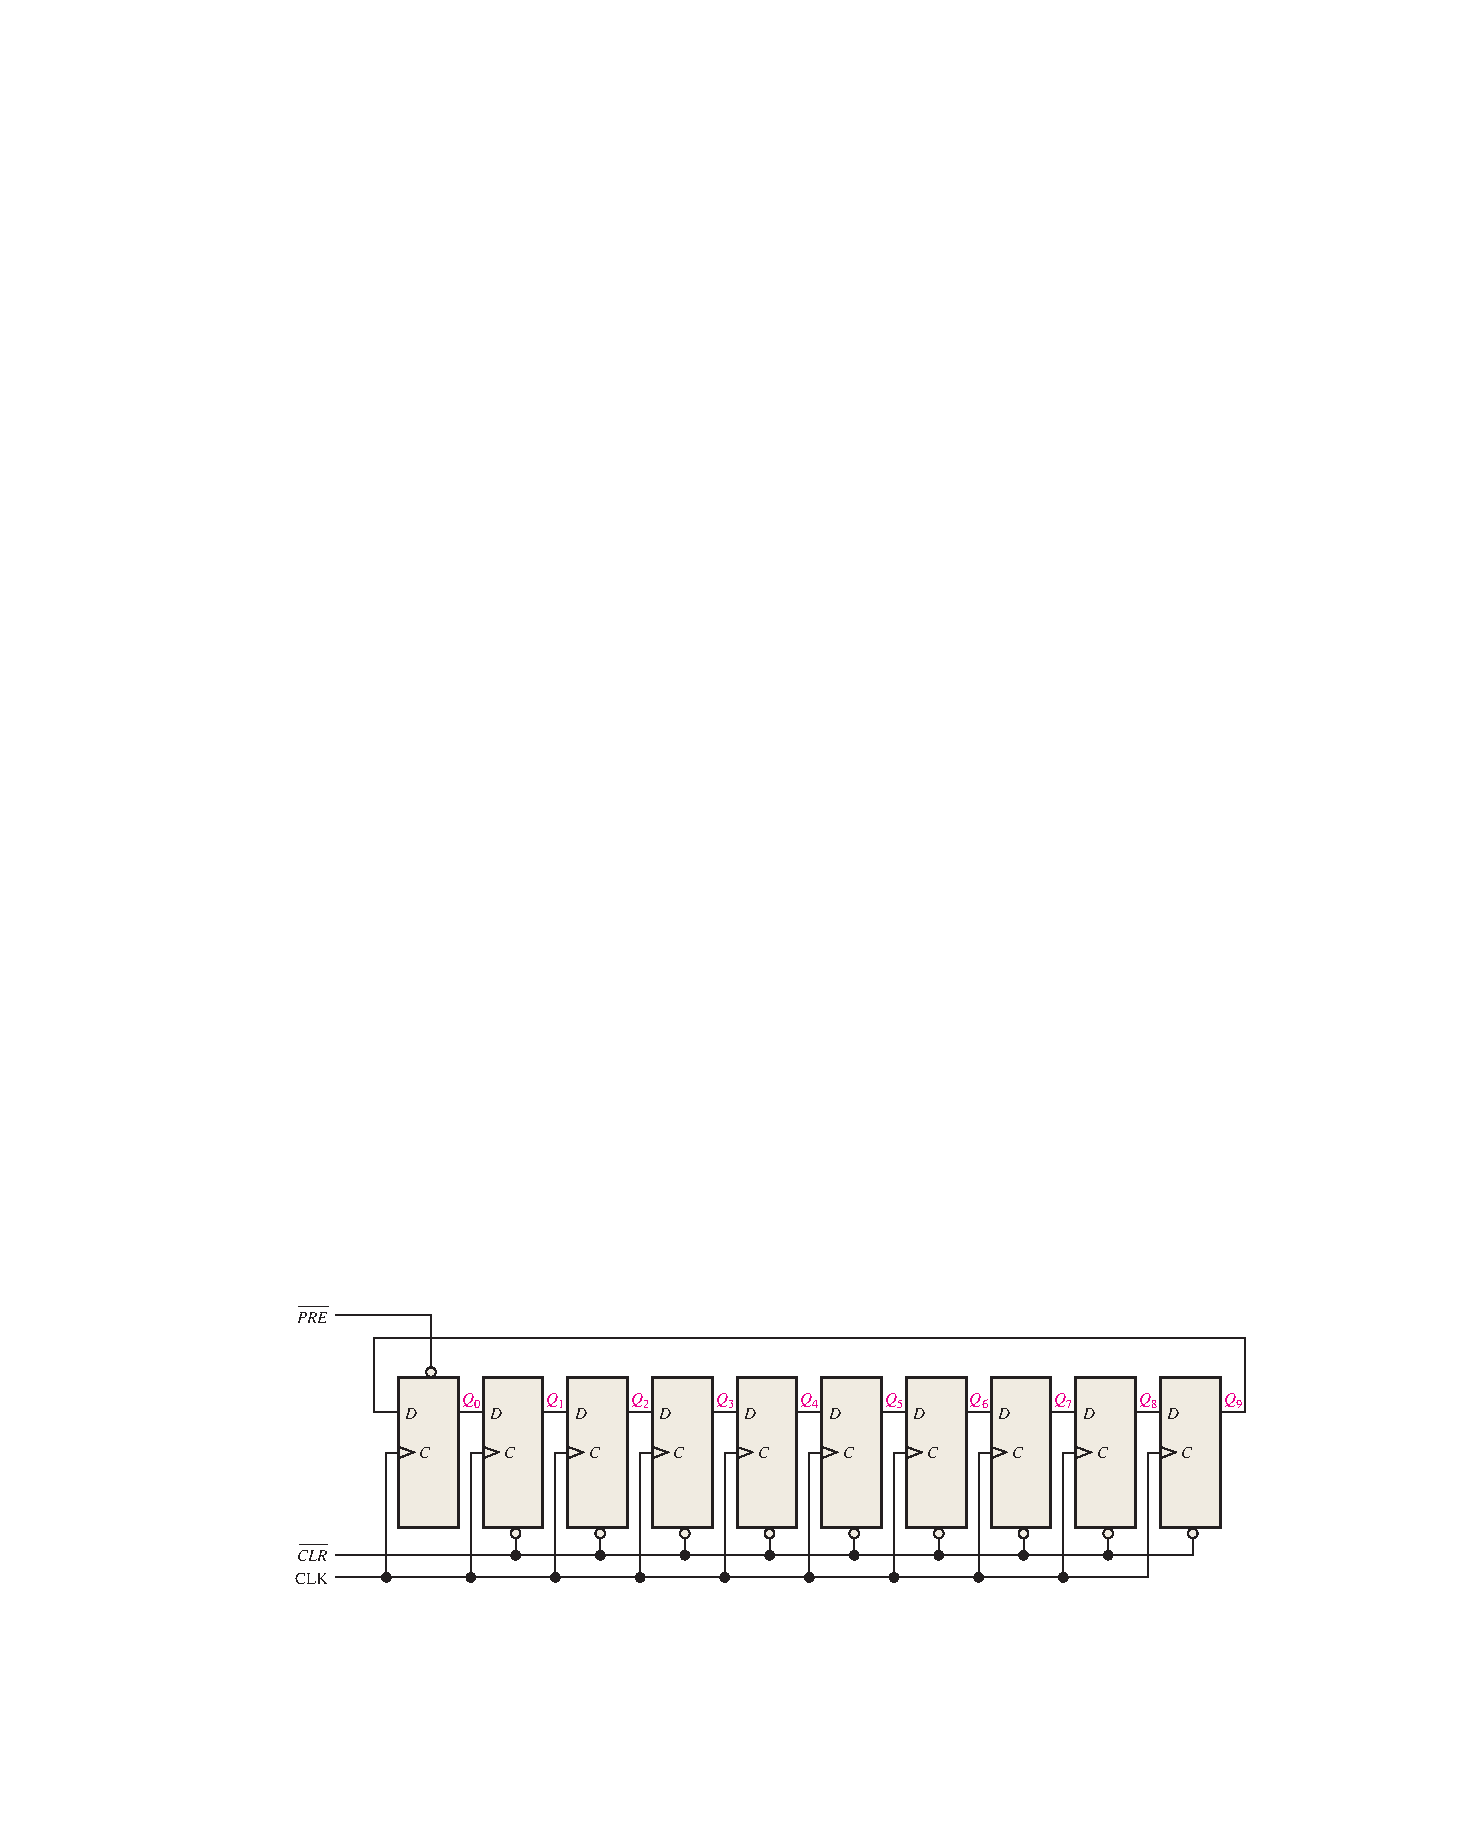
\includegraphics[scale = 0.75]{Graphics/KEYPAD/RING_COUNTER.pdf}
    \caption{10-bit Ring Counter ~\autocite{FLOYD}}
    \label{fig:KEYPAD_RING}
\end{figure}

\medskip
The initialization of the ring counter is done with a pulse coming from the auto start timer that is fed into the \emph{START} input of the GAL, see \textbf{Subsection} \textbf{\ref{sec:ENABLE_AUTOSTART}} for more on this. Once this pulse is detected by the GAL, it introduces a bit in the \emph{l\_temp} internal signal starting the counter. 

\medskip
The \emph{READY} signal is an output that is needed in order to produce the auto start of the system, more on this in \textbf{Subsubsection} \textbf{\ref{sec:AUTOSTART}}.\medskip

Besides, we can also find an output 4 bit array, called \emph{SIG}, which will output the BCD Code that we have previously discussed.\medskip


This I/O configuration can be seen in the following image:\medskip

\begin{figure}[H]
    \centering
    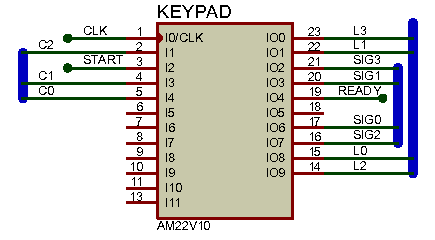
\includegraphics[scale = 1]{Graphics/KEYPAD/KEYPAD_PROTEUS.PDF}
    \caption{Proteus Subassembly of Keypad}
    \label{fig:KEYPAD_PROTEUS}
\end{figure}

\clearpage

The VHDL code that we used for this part of the system is very similar to the one that we used in the practical sessions. It can be found below: 

\vspace{0.5cm}

\inputcode{Code/KEYPAD.vhd}

\subsection{Memory device}

The auxiliary memory of a system has the duty of keeping essential information that the Central Processing Unit (CPU), in our case a GAL, will need in order to operate.

\medskip
This information is usually kept in words of two bytes (16 bits in total), treated as individual entities or memory locations.


In order to increment the amount of data that can be stores, memory devices combine multiple memory locations into two dimensional arrays (i.e. 8x8 array), or even three dimensional arrays (i.e. 8x8x8 array). We can see this here:

\begin{figure}[H]
    \centering
    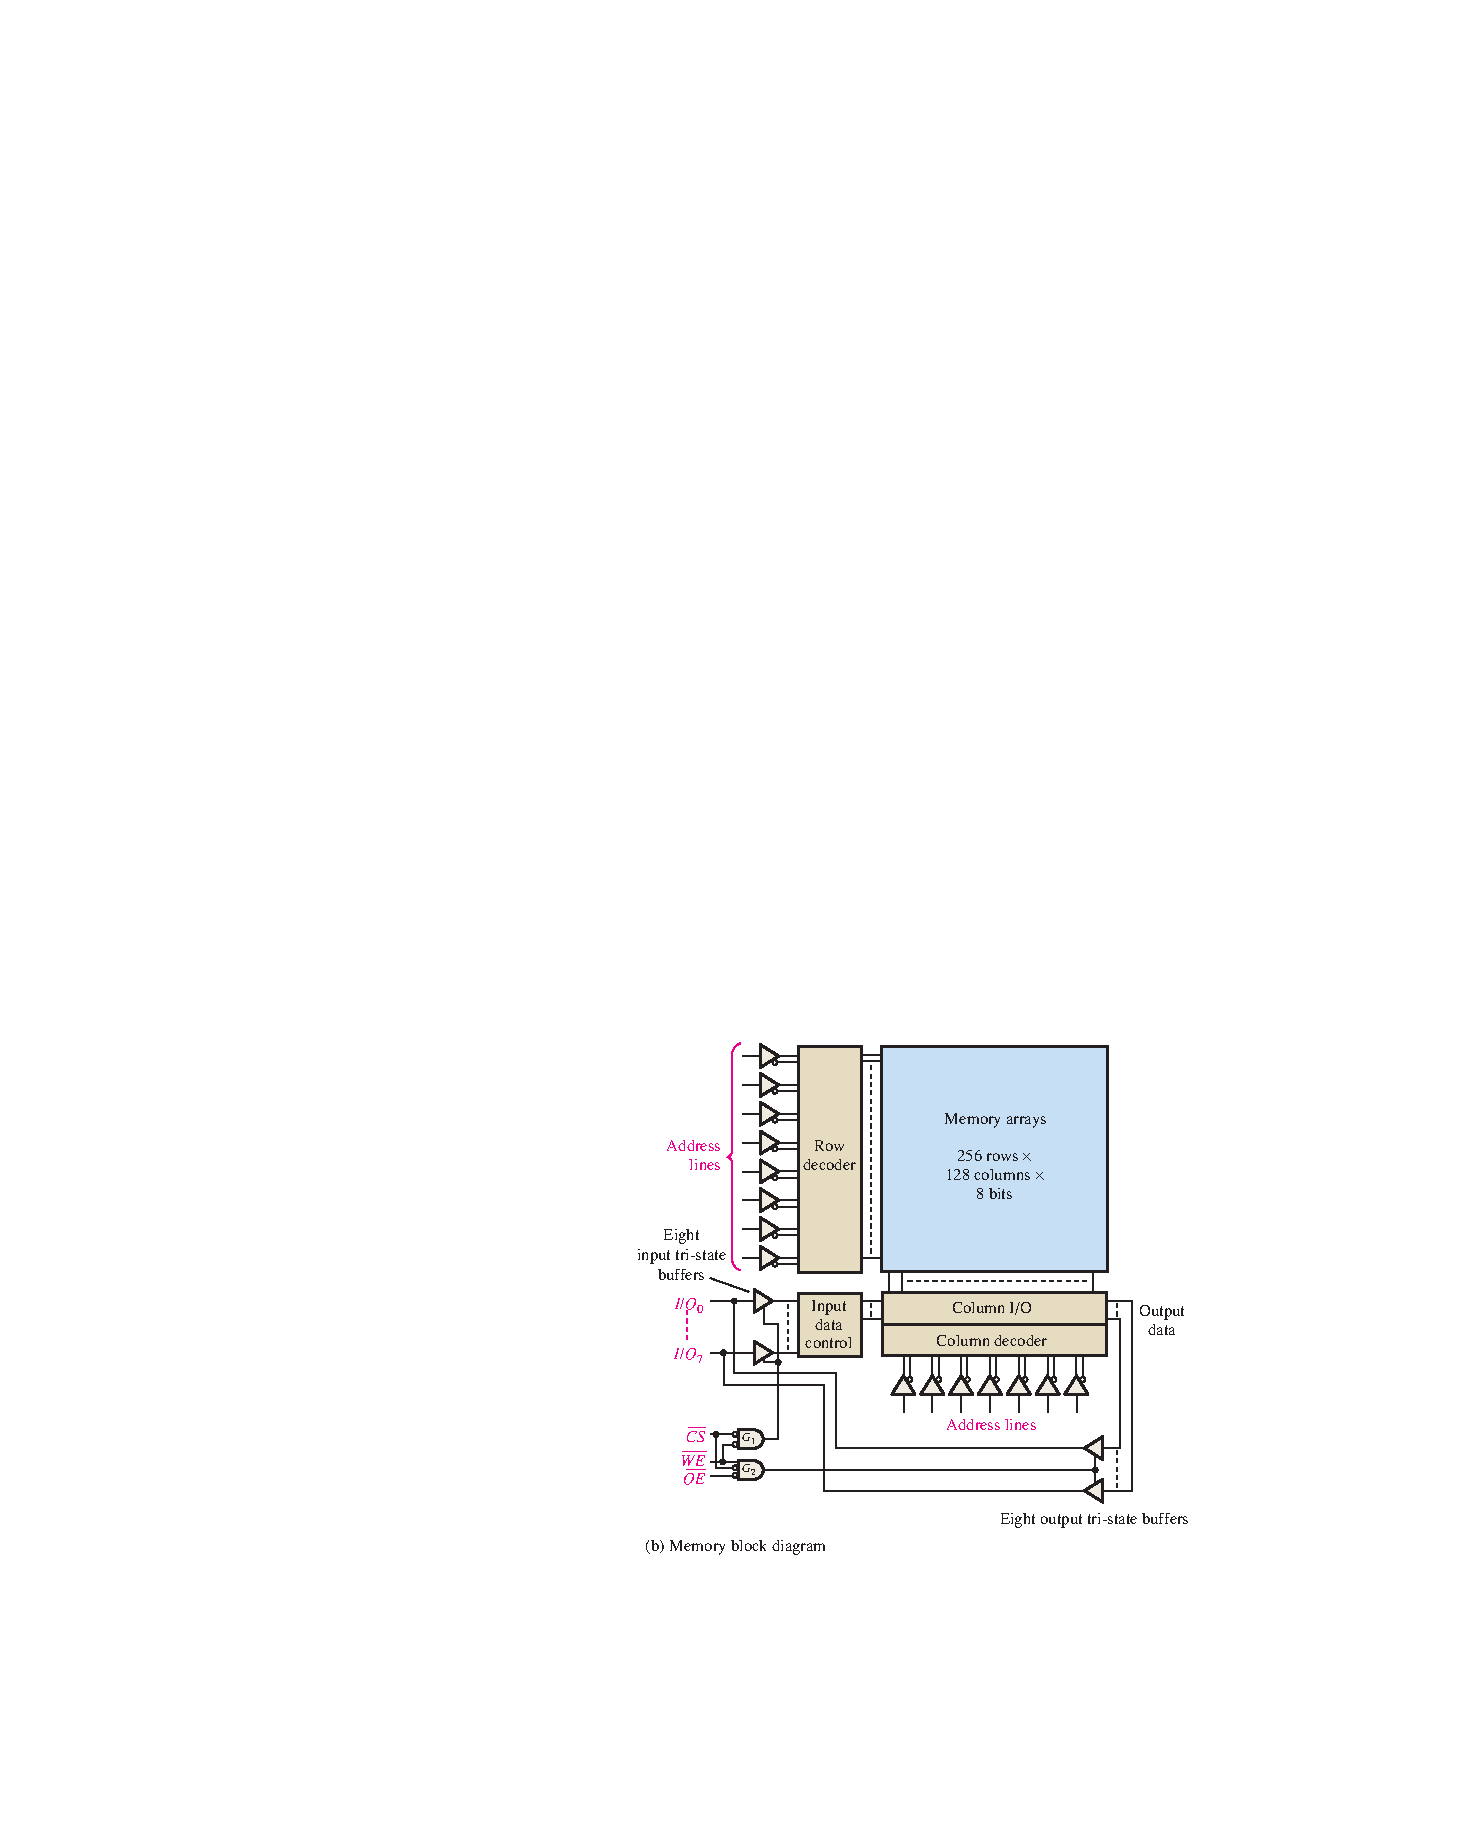
\includegraphics[scale = 0.85]{Graphics/RAM/RAM_BLOCK_DIAG.pdf}
    \caption{RAM block diagram ~\autocite{FLOYD}}
    \label{fig:RAM_BLOCK_DIAG}
\end{figure}


\begin{figure}[H]
    \centering
    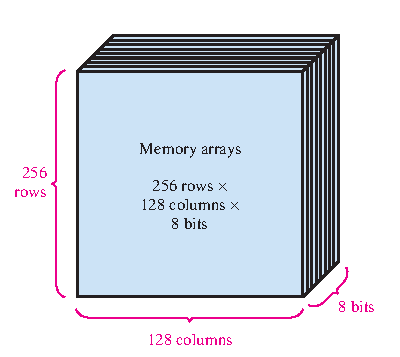
\includegraphics[scale = 0.85]{Graphics/RAM/RAM_BLOCK_CONFIG.pdf}
    \caption{RAM array configuration ~\autocite{FLOYD}}
    \label{fig:RAM_BLOCK_CONFIG}
\end{figure}


\subsubsection{Chip description}

\medskip
\hspace{0.5cm}
{\large \textit{\textbf{Chip Enable}}}
\medskip

To operate the memory first we have to activate the Chip Enable $\overline{CE}$  terminal (Active Low). \medskip

When a CPU has to handle multiple memory chips, in order to read or write from one of them, the other ones are disabled sending a HIGH to their respective $\overline{CE}$ terminals. 

\medskip
{\large \textit{\textbf{Write Enable}}}
\medskip

With this terminal the CPU specifies if the operation it wants to execute is to write into the memory (LOW at $\overline{WE}$) or to read from the memory (HIGH at $\overline{WE}$).

\medskip
{\large \textit{\textbf{Output enable}}}
\medskip


The $\overline{OE}$ connects the output of the memory to the data bus. If it is in LOW, data can be sent from the memory. Otherwise, a HIGH level will create a High-Z output at the Data Bus.  We usually keep it in a constant LOW in order to simplify the system.

\medskip
{\large \textit{\textbf{Address bus}}}
\medskip


In order to read or write, the GAL must first specify which memory location it wants to work with. This is done by means of the address bus, corresponding to the row and the column of the memory matrix. 

\begin{table}[H]
    \centering
        \begin{tabular}[t]{lccccc}
            \toprule
            & \textbf{Mode} & $\mathbf{\overline{CS}}$ & $\mathbf{\overline{OE}}$ & $\mathbf{\overline{WE}}$ & \textbf{I/O}\\
            \midrule
                &    Standby   &    H   &   X   &   X   &   High-Z        \\
                &    Read      &    L   &   L   &   H   &   $\text{DATA}_{OUT}$    \\
                &    Read      &    L   &   H   &   H   &   High-Z        \\
                &    Write     &    L   &   X   &   L   &   $\text{DATA}_{IN}$     \\
            \bottomrule
        \end{tabular}
        \caption{Operation Modes Truth Table ~\autocite{6116}}
        \label{table: RAM_MODES}
\end{table}


The RAM device used in the project is the 6116, a 16K (2048 x 8 bit) high speed memory chip.

In order to simplify the operation, as only 4 digits are stored, we will only use the A0 and A1 Address terminals. 

Also, as we only need to store digits from 0 to 9, only the first 4 bits of the Data Bus will be used.

\subsection{Safecode}

\subsubsection{Writing Operation}
\label{sec:WRITING_OPERATION}

In order to be able to check the introduced password, we will program it into a Random Access Memory (RAM), in particular a 6116 CMOS Static one so as to be able to read it later on. To do this, we will use a GAL. In this case, the clock (CLK) and the BCD signal from the KEYPAD GAL (SIG) will be its inputs. In order for the RAM to work properly, it requires the SAFECODE GAL to have as output a Chip Select signal (CS\_\_), an Address signal (A), and the BCD (D\_\_).\medskip

As the programmable chip acts as a FSM, it will also have as output a representation of its current state, which will be later used to command other GAL devices. It should be noted that due to the fact that the RAM IC will be commanded by different GALs, we have added resistors between the output of the GAL and the control pins of the RAM so as to avoid short circuits. We can clearly see this in the following picture:

\begin{figure}[H]
    \centering
    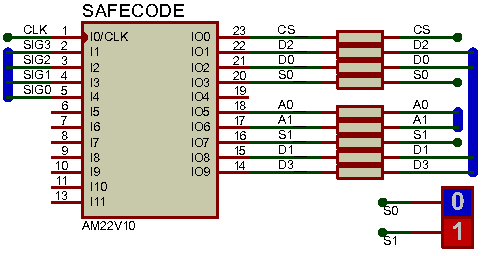
\includegraphics[scale = 1]{Graphics/SAFECODE/SAFECODE_PROTEUS.PDF}
    \caption{Proteus Subassembly of Safecode}
    \label{fig:SAFECODE_PROTEUS}
\end{figure}


\medskip
The memory device will start storing data when the Write Enable ($\overline{WE}$) signal and the Chip Select ($\overline{CS}$) are pulled LOW by the GAL. A timing diagram is attached:\medskip

\begin{figure}[H]
    \centering
    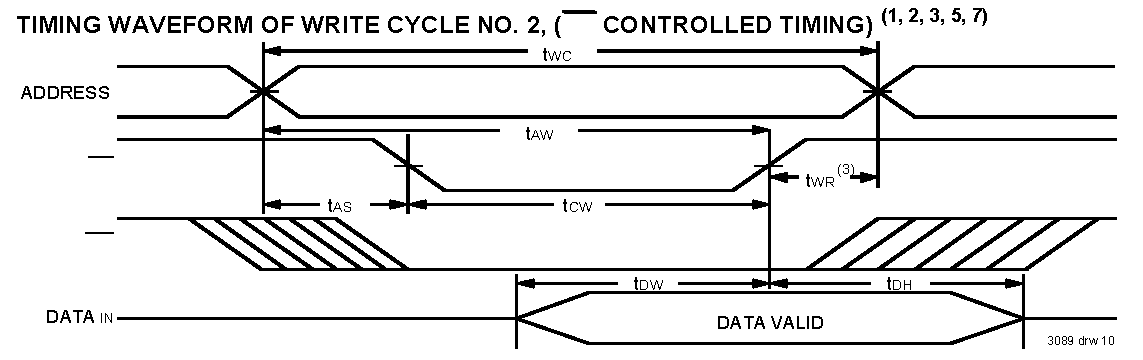
\includegraphics[scale = 0.60]{Graphics/RAM/6116.pdf}
    \caption{6116 RAM Write Cycle}
    \label{fig:6116}
\end{figure}


The general truth table of this specific RAM, though it is mostly the same for most RAM chips, can be found in \textbf{Table} \textbf{\ref{table: RAM_MODES}} \medskip

Now we will discuss the different states that we have defined in our FSM. As per before, the full code will be attached as well.

\subsubsection{FSM States Overview}

    \hspace{0.4cm}
    \bm{$Q_0$}
\medskip

At rest, the system must start at Address "00", and the $\overline{CS}$ signal must be HIGH because it is active when it is LOW. Once the $*$ button is pressed, system transitions to $Q_1$ state.

\medskip
    \bm{$Q_1$}
\medskip

The $\overline{CS}$ signal changes to a LOW level, and the RAM device is in the “ready to write” State $Q_1$. This means that from now on, Address number $00$ is ready to be overwritten by the character we introduce with the keypad. 

\medskip
When introducing a new character with the keypad, the $*$ will make the system stay at $Q_1$,  the \textit{\#} character will make the system to return to $Q_0$, and any other character will make the system change to State $Q_2$. \medskip

\bm{$Q_2$} \textbf{\&} \bm{$Q_3 \textit{\textbf{ and return to }} Q_0$}\medskip

In state $Q_2$, the character previously introduced is written on the address $00$.

\medskip
Now, there are two options: to keep writing on the memory, or to stop writing.


\begin{itemize}
    \item In order to keep writing, any key pressed but \textit{\#} and the same key, will transition the system to state $Q_3$, where the system jumps to the next Address (where the next character will be kept), and the writing loop starts again at \textit{$Q_1$}.
    
    \item In order to stop, the  \textit{\#} button is pressed, and the system returns to state \textit{$Q_0$}, meaning that  the Address is reset to $00$, and the writing operation ends.
\end{itemize}

\clearpage

To illustrate the different states and the transitions between them we have included the following diagram:

\begin{figure}[H]
    \centering
    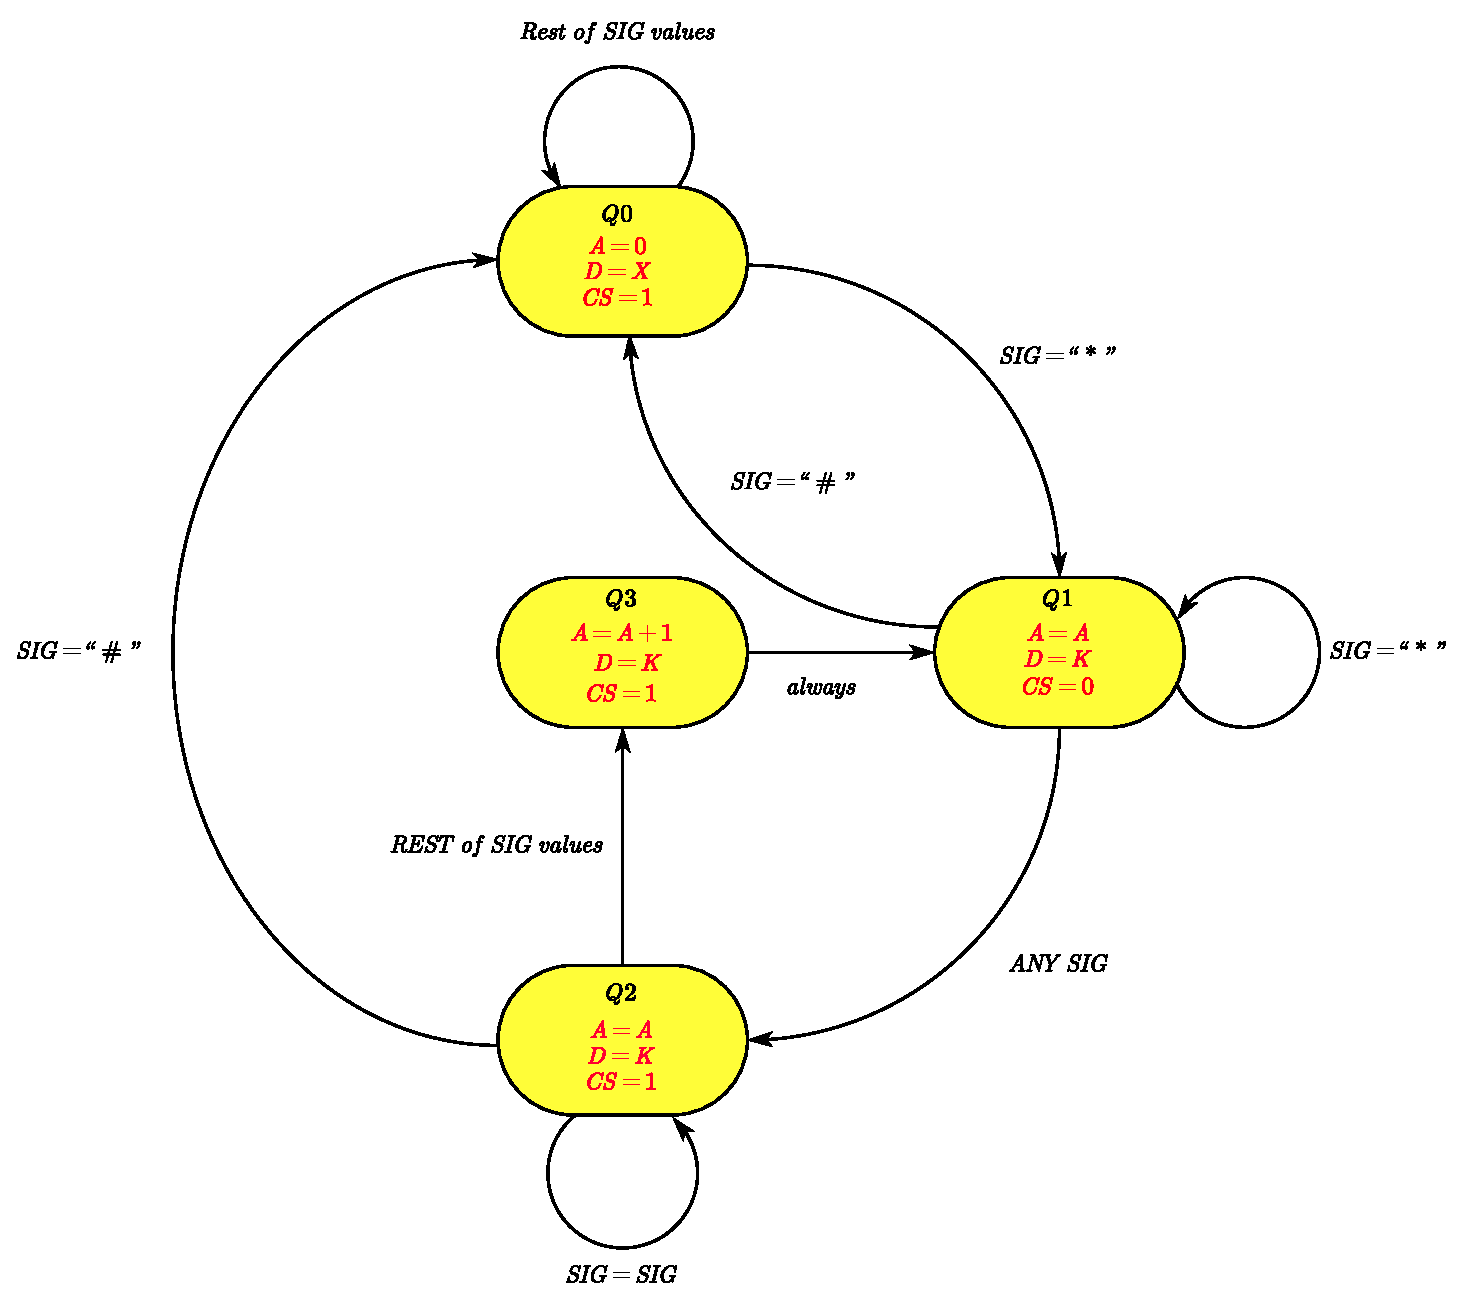
\includegraphics[scale = 0.55]{Graphics/SAFECODE/SAFECODE.pdf}
    \caption{Safecode FSM}
    \label{fig:SAFECODE_FSM}
\end{figure}

The VHDL code for this GAL can be found below:

\inputcode{Code/SAFECODE.vhd}
            


\subsection{State\_Fsm \& Display}

Once the password has been entered, it is displayed in the 4 7-segment displays. This display must show the entered four digit password and the “Open” or “Error” messages, depending on whether code is correct or not. Since all of the checking/validating code cannot fit in one GAL. the display must be able to be controlled by different GAL devices.\medskip

In order to display the entered password, two different GALs, State\_FSM and Display, will be used due to the length of the code. We will go over the "Open"/"Error" messages later.\medskip


{\subsubsection{State\_Fsm} }
\medskip

STATE\_FSM has as input the clock (\textit{CLK}), the \textit{RESET} signal, the output FSM states from the SAFECODE (\textit{S}) as inputs as well (As we discussed in \textbf{Subsubsection \ref{sec:WRITING_OPERATION}}), and the \textit{DONE} signal as output. \medskip

Most of the GALs of this project use FSMs to command the different operations, including this one. We will now go over the different states that form the State Machine:

\medskip
    \bm{$Q_0$}
\medskip

Initially, \textit{DONE}  is in a LOW level, then, the Final State Machine begins. The first state, \textit{$Q_0$}, pulls \textit{DONE} LOW, and changes to the next state if the read state from the safecode \textit{S} $= 00$. 

\medskip
{\textbf{\textit{\bm{$Q_1$}, \bm{$Q_2$} and return to \bm{$Q_0$}}}}
\medskip

At \textit{$Q_1$}, DONE remains the same, and once \textit{S} $= 10$, that is, the second state of the SAFECODE, DONE is pulled HIGH and the state changes to \textit{$Q_2$}. No changes occur in \textit{$Q_2$} until RESET is in HIGH level, then the state becomes \textit{$Q_0$}, effectively resetting the GAL.

\clearpage

To illustrate the different states and the transitions between them we have included the following diagram:\medskip

\begin{figure}[H]
    \centering
    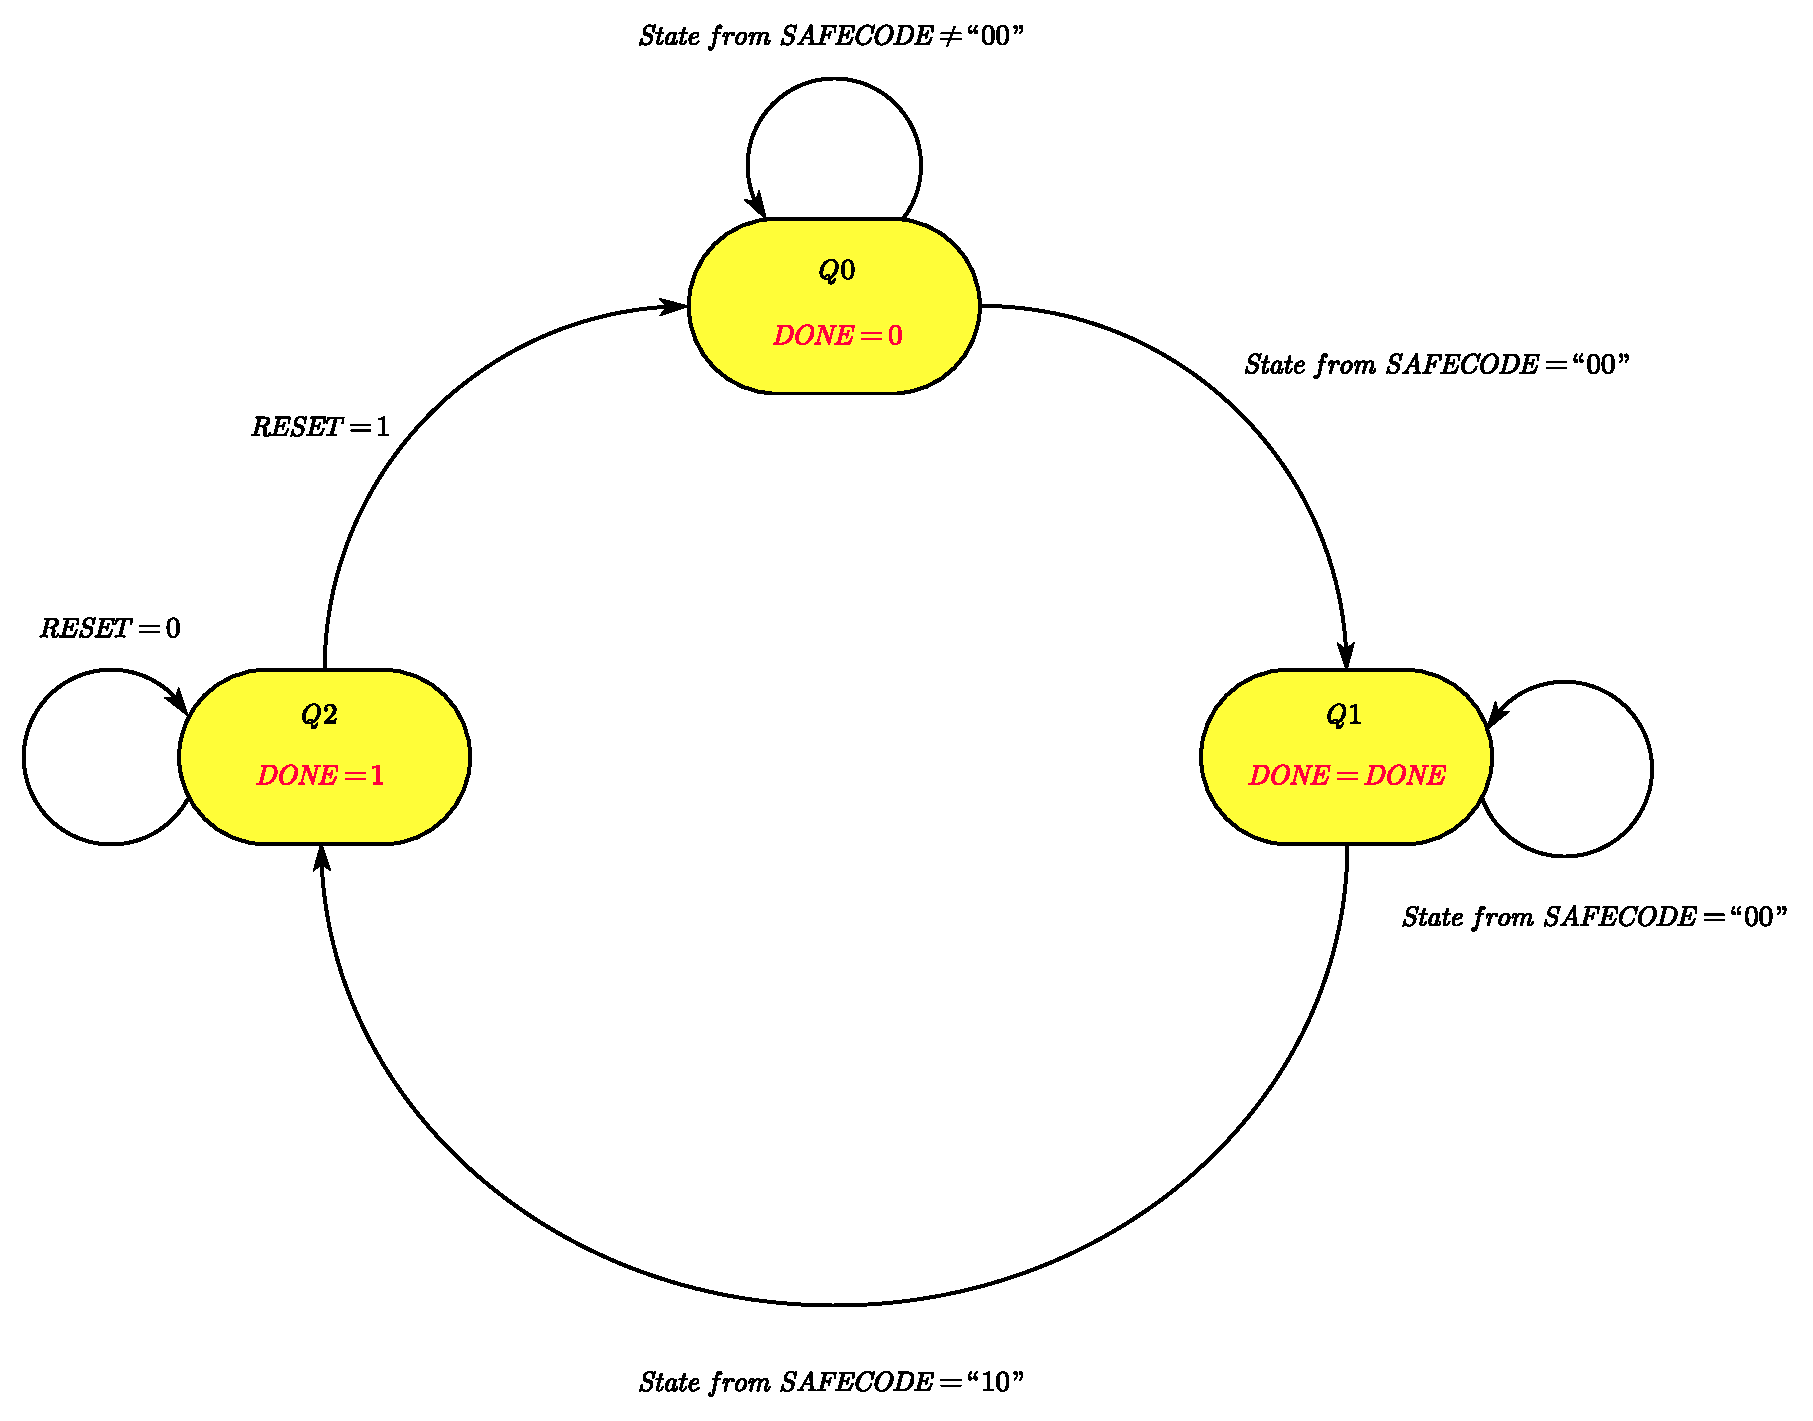
\includegraphics[scale = 0.49]{Graphics/STATE_FSM + DISPLAY/STATE_FSM.pdf}
    \caption{State\_FSM FSM}
    \label{fig:STATE_FSM_FSM}
\end{figure}

\vspace{0.6cm}

The VHDL code for this GAL can be found below: \bigskip

\inputcode{Code/STATE_FSM.vhd}


\clearpage

\subsubsection{Display}
\label{sec:DISPLAY}

DISPLAY has, as an input, the clock signal (\textit{CLK}) and \textit{DONE} signal from STATE\_FSM. Also, it has as outputs \textit{SEL}, a 4 bit signal which acts as a ring counter for the 4 digit 7 segment displays, \textit{A\_OUT}, a 2-bit vector that controls the addressing of the RAM,  \textit{WE\_OUT} and \textit{CS\_OUT}, being the Write Enable and Chip Select commanding signals for the RAM module.\medskip

Due to the fact that there is more than one GAL connected to the RAM to both read and write to it, as well as to the display, the use of tri-state buffers is necessary so as to avoid short circuits. The tri-state buffers act as switches commanded by CS\_OUT,  A\_OUT \& WE\_OUT. The output of these “switches” are the $\overline{CS}$, A \& $\overline{WE}$ signals needed to control the RAM IC.\medskip

We will now go over the different states that form this Finite State Machine:\bigskip

\textbf{Initialization Stage}\medskip

Every time that DONE is in LOW level, all the outputs are initialized at ‘0’. \medskip

\textbf{Ring (\textit{\bm{$Q_0$}, \bm{$Q_1$}, \bm{$Q_2$}, \bm{$Q_3$}})}
\medskip

Once DONE changes its value to HIGH,  WE\_OUT and CS\_OUT switch to HIGH level as well, enabling the tri-state buffers and pulling $\overline{WE} = 1$ and $\overline{CS}=0$ in order to put the RAM into Read Mode so as to show, at [D0...D3] the corresponding number depending on the address A\_OUT.\medskip

So, in the FSM of this GAL, in each of the states, A\_OUT will have a value for an address, at the same time, SEL will change the position of its HIGH level bit, turning one of the 4  7-segment display ON at a time, with the rest being OFF. Since the clock frequency is high, displaying only one number per clock frequency is enough to trick the human eye into believing that the 4 numbers are being displayed at the same time. This is done in such a way that the sequence of numbers that are being shown correspond to the ones stored in the RAM.\medskip

\medskip
{ \textbf{End of Ring}}
\medskip

If the ring passes through \textit{$Q_0$} and the DONE signal is in a LOW level, the ring stops and the system returns to the initialization stage.  


To show the numbers in the display, we have fashioned a custom 7-segment display driver. We can see it in the following image:

\begin{figure}[H]
    \centering
    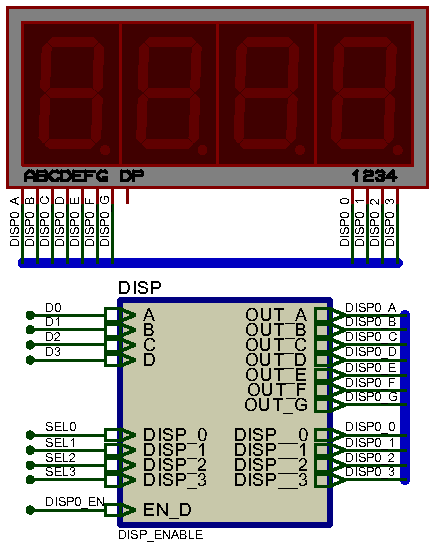
\includegraphics[scale = 0.9]{Graphics/STATE_FSM + DISPLAY/DISP_ENABLE.PDF}
    \caption{Proteus Subassembly of 7-segment display driver}
    \label{fig:DISP_ENABLE}
\end{figure}

The internals of this driver are composed of a 74247 display driver and some tri-state buffers to control when the driver is on, as well as to prevent short circuits in the outputs of the driver/inputs of the display. As we said before, this is due to the fact that the display is driven by different GALs, so we want a High-Z output in the drivers that are not in use. The \textit{EN\_D} signal is provided by another GAL that takes care of selecting which signal to display. (See \textbf{Subsubsection} \textbf{\ref{sec:ENABLE_SEL}} for more on this). We can see this internals here:

\begin{figure}[H]
    \centering
    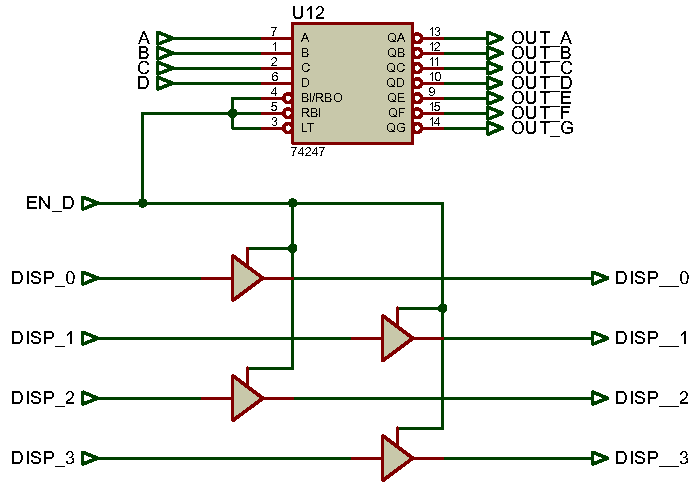
\includegraphics[scale = 0.8]{Graphics/STATE_FSM + DISPLAY/DISP_ENABLE_INT.PDF}
    \caption{7-segment display driver internals}
    \label{fig:DISP_ENABLE_INT}
\end{figure}

\clearpage

To illustrate the different states and the transitions between them we have included the following diagram:\medskip

\begin{figure}[H]
    \centering
    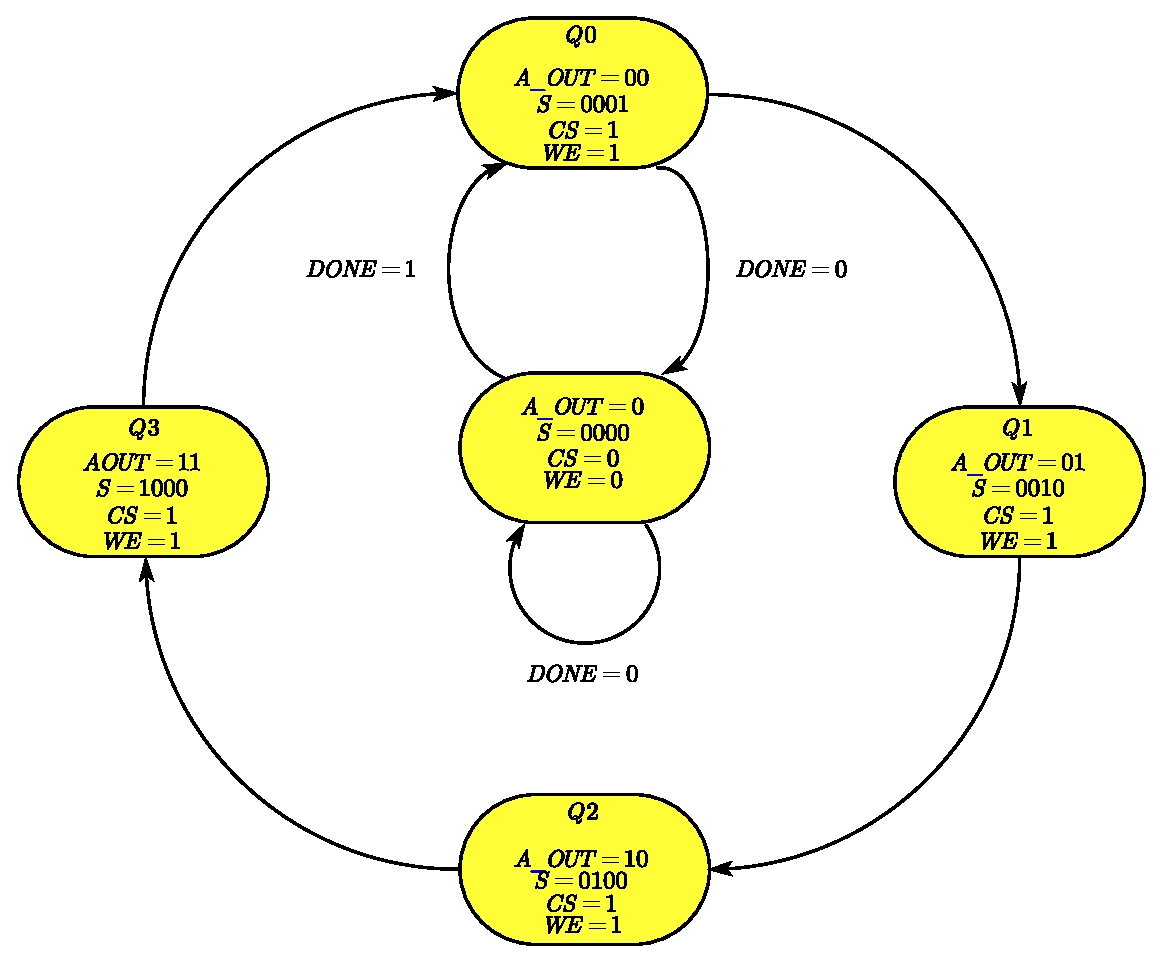
\includegraphics[scale = 0.55]{Graphics/STATE_FSM + DISPLAY/DISPLAY_FSM.pdf}
    \caption{Display FSM}
    \label{fig:DISPLAY_FSM_FSM}
\end{figure}

\vspace{0.5cm}

The final subassembly of both GALs can be seen here:

\begin{figure}[H]
    \centering
    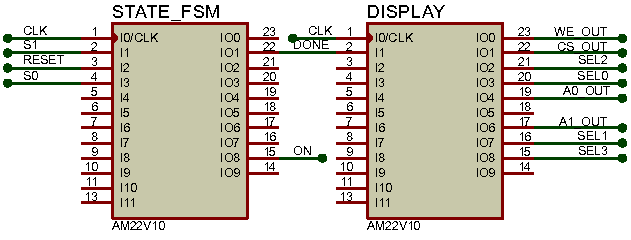
\includegraphics[scale = 1]{Graphics/STATE_FSM + DISPLAY/PROTEUS_BOTH.PDF}
    \caption{Proteus Subassembly of both GALs}
    \label{fig:PROTEUS_STATE_FSM_DISPLAY}
\end{figure}

\clearpage

The VHDL code is attached below:

\vspace{-0.1cm}

\inputcode{Code/DISPLAY.vhd}

\subsubsection{Final Roundup}
\label{sec:STATE_FSM_DISPLAY_ROUNDUP}

We know that this section may strike as a bit complex or hard to understand, so we will try to break down the different actions that both GALs perform in an step by step description of the procedure.

\begin{enumerate}
    \item The STATE\_FSM reads the state of SAFECODE using the state outputs of the latter.
    
    \item Once it detects a "00" it knows that the password is being entered.
    
    \item As soon as it reads a "10" (Last State of SAFECODE, triggered by the \textit{\#} key), it knows that all numbers have been entered and so it turns the \textit{DONE} pin ON.
    
    \item DISPLAY reads the \textit{DONE} pin and as soon as it turns ON, it starts a ring counter that sweeps through the 4 7-segment displays activating one each time. At the same time, the RAM is put into Read mode and the addresses are swept as well. In essence, the first displays turns on (with the rest off) and it displays the contents of Address = "00", then the second display turns on and displays Adress "01", and so on. This happens very fast, tricking the person into believing that all 4 displays are ON simultaneously.
    
    \item Once the \textit{RESET} signal is received by STATE\_FSM, the \textit{DONE} pin is pulled LOW and both GALs are reset.
\end{enumerate}




\subsection{Digit 0, 1, 2, 3}
\label{sec:IND_CHECK}

Once the 4 digit password is entered with the keypad, the system has to compare it with the password preset by the user with the dip-switches.

\medskip

In order to do this, each of the 4 digits of the password is compared by a different GAL due to a limitation in the number of input pins. This example corresponds to the DIGIT\_0 of the password, but the other three work in the same way, thus, only one of them is explained. 

\medskip

For the GAL to know which of the digits is the first one, the Address (A) from the memory device is read. In this case, if the Address is $00$, we have the digit required at the Data Bus (D).\medskip

We will now go over the different states of the Finite State Machine: \medskip

\medskip
\textit{\bm{$Q_0$}}
\medskip

By default, the Output of the GAL, \textit{DIGIT\_0} is at a LOW state. The GAL checks 4 inputs, namely \textit{DONE}, the predefined password (via the dip switch) \textit{PASS0}, the address value, \textit{A} and the value stored in the RAM at that specific address, \textit{D}. If the \textit{DONE} pin is ON, meaning that the whole password has been introduced, the address is "00" (for this particular digit), and \textit{PASS0} = \textit{D}, then the state is changed and the FSM moves to \textit{Q1}.\medskip

\textit{\bm{$Q_1$}}
\medskip

In this state, the GAL device will output a HIGH at \textit{DIGIT\_0} indicating that the first digit of the password is correct. \medskip

Finally, when the \textit{RESET} signal is detected, the state switches back to Q0 and the \textit{DIGIT\_0} pin is pulled LOW, effectively resetting the FSM. \medskip

To illustrate the different states and the transitions between them we have included the following diagram:

\begin{figure}[H]
    \centering
    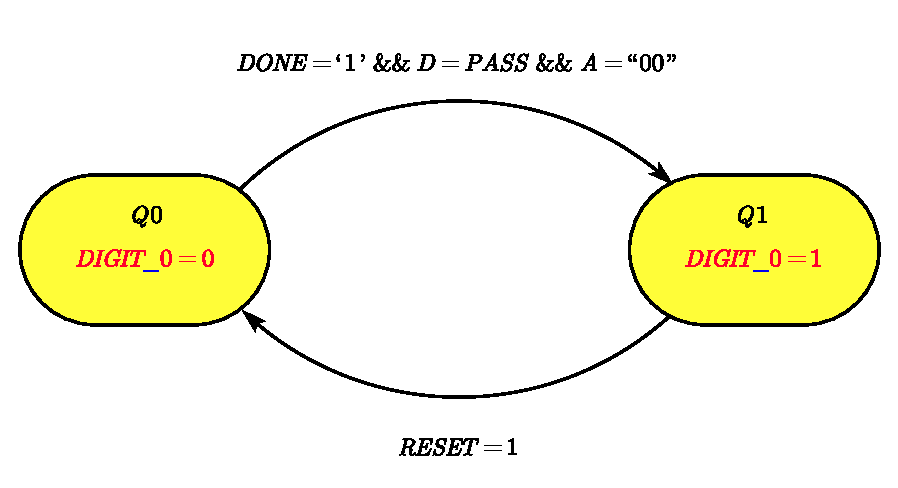
\includegraphics[scale = 0.6]{Graphics/DIGITS/DIGITS_FSM.pdf}
    \caption{Digits [0...3] FSM}
    \label{fig:DIGITS_FSM}
\end{figure}


\clearpage

The VHDL code describing this subsystem is attached below:

\inputcode{Code/DIGITS.vhd}

\clearpage

The Proteus subassembly corresponding to the 4 digits can be seen below:

\begin{figure}[H]
    \centering
    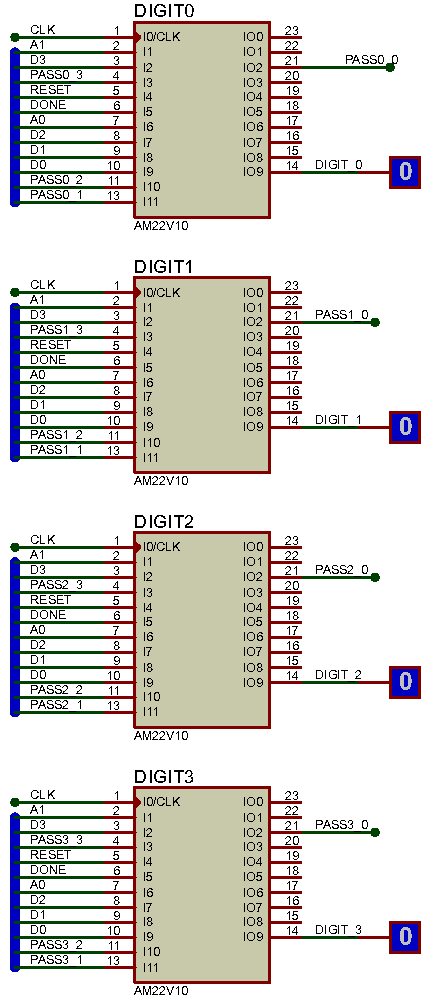
\includegraphics[scale = 1]{Graphics/DIGITS/DIGITS_PROTEUS.PDF}
    \caption{Proteus Subassembly of Digits [0...3]}
    \label{fig:DIGITS_PROTEUS}
\end{figure}



\subsection{Password checking}
\label{sec:PASS_CHECK}

Once every digit has been checked individually, all of them have to be checked to determine whether the whole password is correct or not. To do this, we will make use of another GAL, namely \textit{PASSWORD CHECK}.
\medskip

The latter has as an input, the clock (\textit{CLK}), \textit{DONE\_}, which is the delayed version of DONE (See \textbf{Subsection \ref{sec:DELAYED_STEADY}}), the 4 \textit{DIGIT\_} signals coming from the individual checks and the general \textit{RESET}. As outputs, it has \textit{CORRECT} signal, and \textit{SENT\_PULSE\_}, a signal that is used to initialize the time-sensitive operations which purpose is to display the introduced password in the 4 7-segment displays followed by the \textbf{\textit{Open}}/\textbf{\textit{Error}} message and finally, once everything has been displayed, to reset the whole circuit.\medskip

The \textit{DONE\_} signal is a slighty delayed version of the original \textit{DONE} signal. This is needed because otherwise the individual digit signals, which are normally LOW, arrive \textbf{AFTER} the \textit{DONE} one, creating a point in time in which the \textit{DONE} is \textbf{HIGH}, which would indicate that the password has been entered, but the \textit{DIGIT\_} signals are still \textbf{LOW} since the GALs in \textbf{Subsection \ref{sec:IND_CHECK}} have not had the time to process the digits yet. Delaying the \textit{DONE} signal by some ms, a time higher than the propagation delay of the GALs, solves this problem.\bigskip

We will now go over all the states that form the FSM:

\medskip
    \bm{$Q_0$}
\medskip

The code follows the operation of a FSM with 3 states. In \textit{$Q_0$}, \textit{CORRECT} and \textit{SENT\_PULSE} are initialized as LOW level, and remain in this condition until a HIGH is read in the delayed version of \textit{DONE}, \textit{DONE\_}. Depending on the value of \textit{DIGIT\_} in that moment, the next state will either be \textit{$Q_1$} or \textit{$Q_2$}.\medskip

If all bits of the \textit{DIGIT\_} array are on a HIGH level, it means that every digit stored in the RAM coincides in magnitude and order to the ones stored in the dip switches inside the security box. In this case the next state is \textit{$Q_1$}.\medskip

On the other hand, if all bits of the \textit{DIGIT\_} array are NOT on a HIGH level, the state will change to \textit{$Q_2$}. 

\medskip
    \bm{$Q_1$}
\medskip

If the GAL is in this state, it will pull \textbf{\textit{CORRECT}} and \textbf{\textit{SENT\_PULSE}} \textbf{HIGH} and it will wait for the \textit{RESET} signal. Once received, the state will toggle to \textit{$Q_0$} effectively resetting the GAL.

\medskip
    \bm{$Q_2$}
\medskip

In this state the GAL will pull the \textbf{\textit{CORRECT}} signal \textbf{LOW}, so as to indicate that it is NOT correct, and it will pull the \textbf{\textit{SENT\_PULSE}} \textbf{HIGH}, initializing the time-sensitive sequence that we discussed earlier. As per the last state, when a HIGH is received in the \textit{RESET} pin, the state will toggle to \textit{$Q_0$} effectively resetting the GAL.

\clearpage

To illustrate the different states and the transitions between them we have included the following diagram:

\begin{figure}[H]
    \centering
    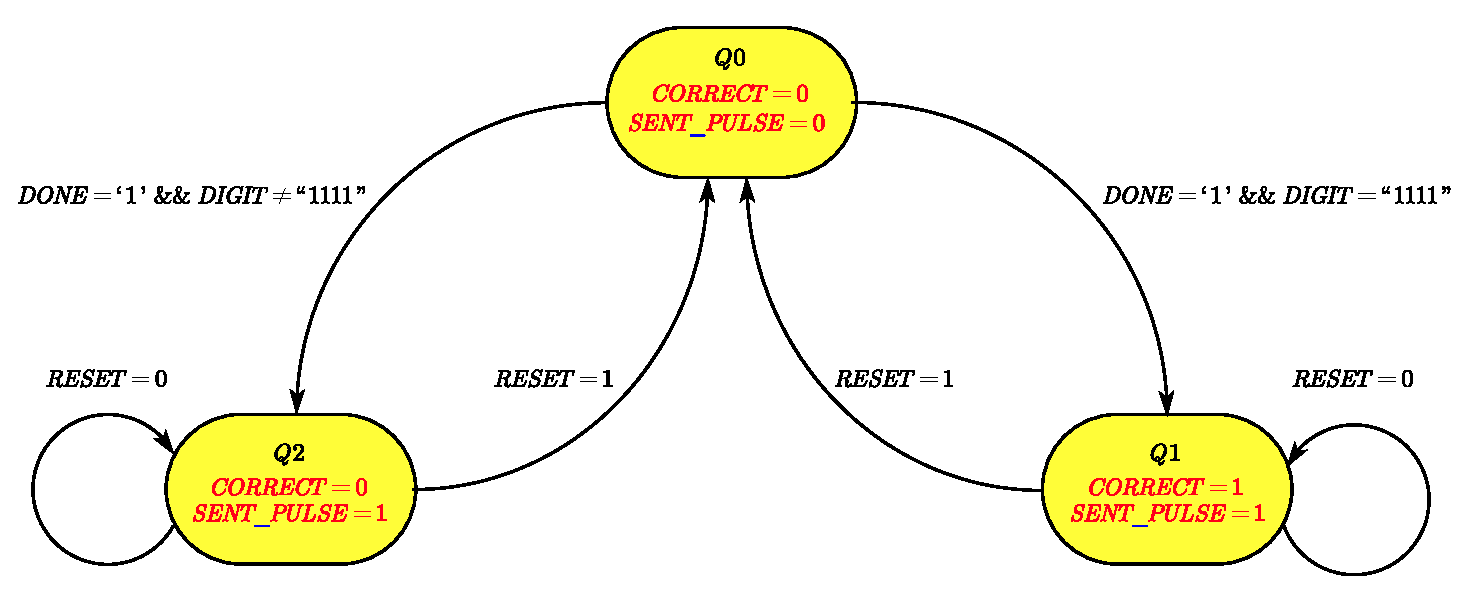
\includegraphics[scale = 0.55]{Graphics/PASSWORD CHECK/PASSWORD_CHECK_FSM.pdf}
    \caption{Password Check FSM}
    \label{fig:PASSWORD_CHECK_FSM}
\end{figure}

\vspace{0.5cm}

The VHDL code describing the operation of the FSM is attached below:

\inputcode{Code/MULTIPLIER.vhd}

Finally, the Proteus subassembly of the circuit can be found below:

\begin{figure}[H]
    \centering
    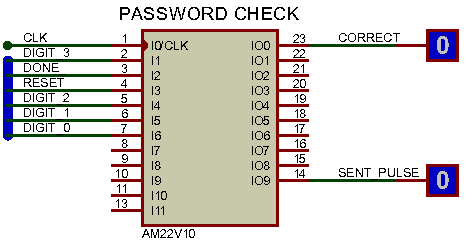
\includegraphics[scale = 1]{Graphics/PASSWORD CHECK/PASSWORD_CHECK_PROTEUS.PDF}
    \caption{Proteus Subassembly of Password Check}
    \label{fig:PASSWORD_CHECK_PROTEUS}
\end{figure}
\subsection{Open/Error Message Displaying}
\label{sec:OPEN_ERROR}

Once the system has determined whether the password entered via the keypad is correct or not, an HMI (Human-Machine Interface) must be implemented. \medskip

In order to do this, we will display the result of the checking process in the 4 7-segment displays that we have already seen. 2 GALs, in combination with some special circuitry that we have fashioned ourselves will be in charge of displaying the messages: Either \textbf{\textit{Open}}, when the code entered is the correct one, or \textbf{\textit{Err}} when it is not.  

\medskip

As we have said before, each message will be processed by one GAL device due to a constraint in the number of pins. We will now go over the code of both GALs and the custom circuitry that allows us to display the messages: \medskip


\subsubsection{\textit{Open} Message}
\label{sec:OPEN_MESSAGE}

As per most of the GALs that we have used, both of them use a FSM to command the different operations. Since the codes of both are almost equal, the I/O declaration of pins will be the same. \medskip

On the one hand, as an input, we may find the signals clock (\textit{CLK}), the \textit{DONE} signal (Not the delayed version this time), the \textit{CORRECT} signal, which we thoroughly discussed in \textbf{Subsection \ref{sec:PASS_CHECK}}, the \textit{INCOMING\_PULSE} signal, which is a delayed pulse of the signal \textit{SENT\_PULSE} that again, we discussed in \textbf{Subsection \ref{sec:PASS_CHECK}} and finally, the \textit{RESET} signal, which will reset the FSM back to the original state. \medskip

On the other hand, as an output, we may find the signals \textit{NUMBER} which control the message displaying process, the \textit{DISP\_EN}, which, as the name suggests, enables the display and, finally, \textit{ENDPULSE\_SEND} which resets the whole system after a few ms, so as to allow the user to visualize the Open/Error message for a brief amount of time (See \textbf{Subsection \ref{sec:DELAYED_PULSE}} for more on this). Otherwise, the whole Opening/Error sequence would happen too fast for the user to notice.\medskip

As we have said, the 2 GALs have almost identical codes, that is why we are only going to describe their FSM once. For instance the \textit{OPEN} GAL's FSM can be broken down into the following states:\medskip

\hspace{0.4cm}
\textit{\bm{$Q_0$}} \medskip

The system initializes with \textit{ENABLE} and \textit{ENDPULSE\_SEND\_O} in a LOW level.
Only if \textit{DONE},  the \textit{CORRECT} and the \textit{INCOMING\_PULSE} pins are in a HIGH state, the system will change to the next state, \textit{$Q_1$}.\medskip


\textit{\bm{$Q_1$}, \bm{$Q_2$}, \bm{$Q_3$} \textbf{\&} \bm{$Q_4$}}
\medskip

When the system enters in the \textit{$Q_1$} state, a ring counter starts. As per the DISPLAY GAL, this counter sweeps across the 4 7-segment displays activating only one at the time at very high frequency, enough to make the illusion that the four displays are ON at the same time.\medskip

\clearpage

The only issue that we ran into was displaying the words \textit{Open}/\textit{Err}, due to the pin limitations of the GALs and their small capacity. To solve this, we created our own drivers using a combination of tri-state buffers to provide power to the needed segments out of the 7 available for each particular letter. We can see this here: \medskip 

\begin{figure}[H]
    \centering
    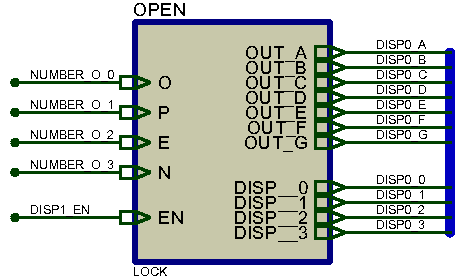
\includegraphics[scale = 1]{Graphics/OPEN-ERROR/OPEN-PARENT.PDF}
    \caption{Custom Fixed Open Message Driver}
    \label{fig:OPEN_DRIVER_PARENT}
\end{figure}

\begin{figure}[H]
    \centering
    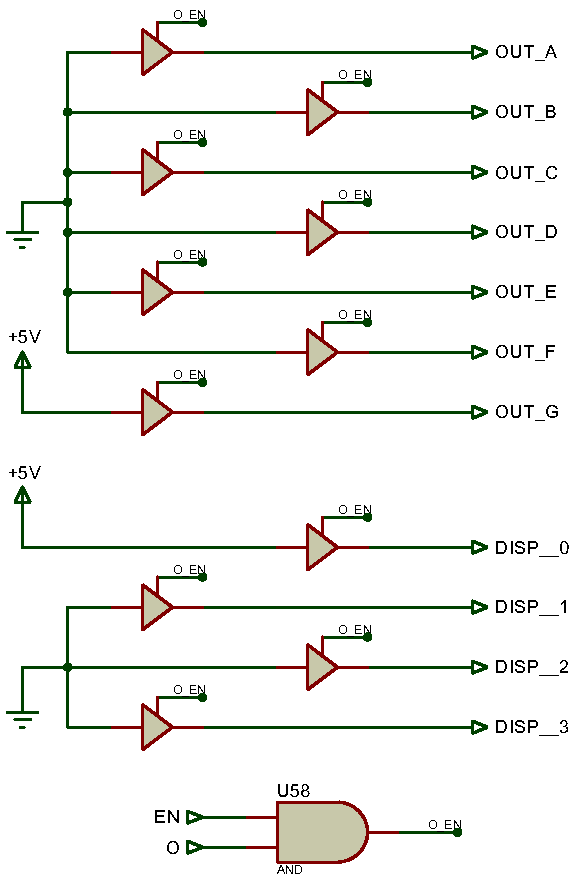
\includegraphics[scale = 0.8]{Graphics/OPEN-ERROR/OPEN-CHILD.PDF}
    \caption{Driver internals (Letter "O")}
    \label{fig:OPEN_DRIVER_CHILD}
\end{figure}

\medskip

These drivers take the \textit{NUMBER} signal as well as the ENABLE SELECTOR's \textit{ENABLE} one as inputs. When the GALs starts the ring, the \textit{ENABLE} signal is pulled HIGH, and based on the choice of the \textit{ENABLE SELECTOR} GAL (See \textbf{Subsection \ref{sec:ENABLE_AUTOSTART}} for more on this topic) the driver outputs both the display address, i.e., which 7-segment display needs to be turned on, as well as the state of the 7 segments. This allows us to create custom messages using a reduced amount of pins.\medskip

Of course, this method is rudimentary and not very efficient nor cost effective, but it was necessary for the correct visualization of the data.\medskip

To conclude, each time that the ring passes through \bm{$Q_4$}, i.e., the state corresponding to letter \textit{N}, the system checks the level of the \textit{RESET} signal. If it is in a HIGH level, the ring finishes and returns to state \textit{$Q_0$}. If it is on a LOW level, the loop continues. This effectively resets the GAL once the message displaying procedure is finished.\medskip

To illustrate the different states and the transitions between them we have included the following diagram:\medskip

\begin{figure}[H]
    \centering
    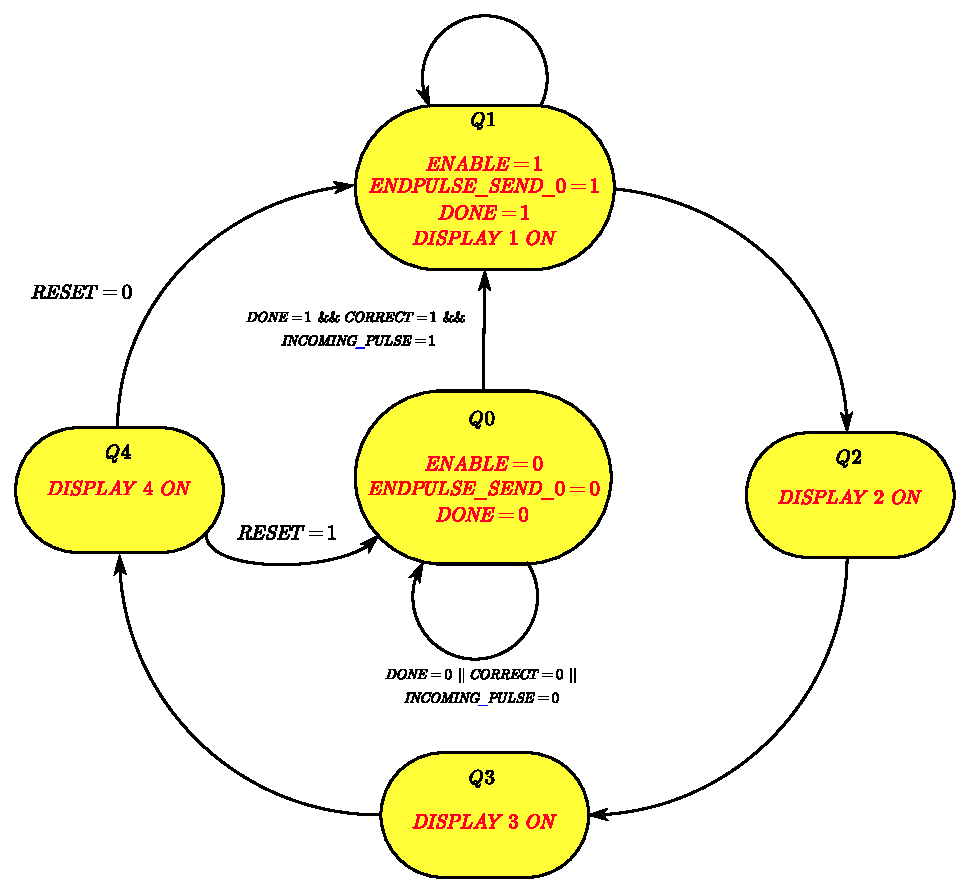
\includegraphics[scale = 0.75]{Graphics/OPEN-ERROR/OPEN_FSM.pdf}
    \caption{Open FSM}
    \label{fig:OPEN_FSM}
\end{figure}

\clearpage

The VHDL code that describes the process can be seen below:

\inputcode{Code/OPEN.vhd}

\clearpage

\subsubsection{\textit{Error} Message}
\medskip

The \textbf{\textit{Error}} message works in the same way as the \textbf{\textit{Open}} message, though there are two main differences:\medskip

\begin{itemize}
    \item The \textit{CORRECT} signal must be in a LOW level as we have to display the error message when the password entered by the user is incorrect.
    \item As the \textbf{\textit{Err}} message has three characters and not four, the fourth display and therefore the last state \textit{$Q_4$} are not used.
\end{itemize} \medskip

To illustrate the different states and the transitions between them we have included the following diagram:\medskip

\begin{figure}[H]
    \centering
    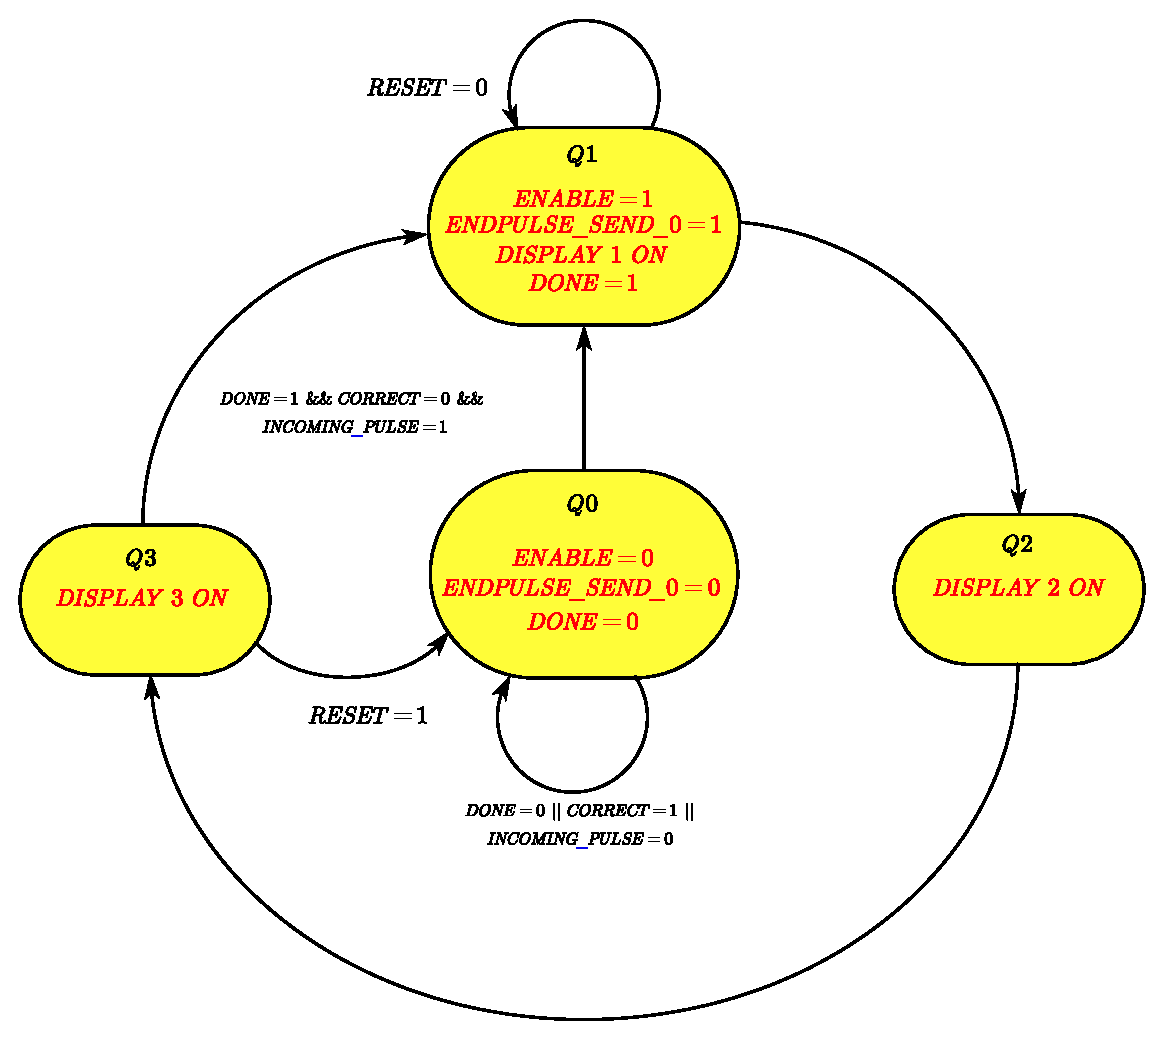
\includegraphics[scale = 0.6]{Graphics/OPEN-ERROR/ERROR_FSM.pdf}
    \caption{Error FSM}
    \label{fig:ERROR_FSM}
\end{figure}

\clearpage

The VHDL code that describes the process can be seen below:

\inputcode{Code/ERROR.vhd}

The Proteus Subassembly of both circuits is attached below:

\begin{figure}[H]
    \centering
    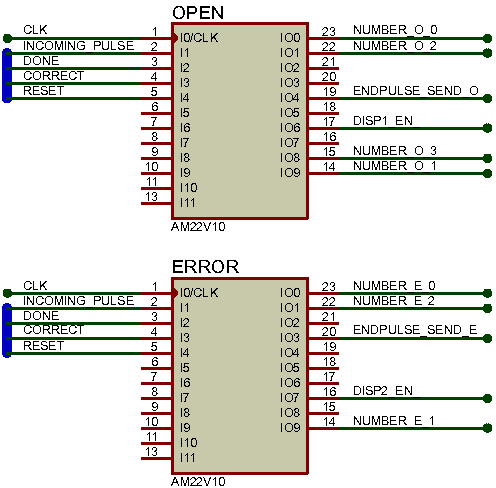
\includegraphics[scale = 1]{Graphics/OPEN-ERROR/OPEN_ERROR_PROTEUS.PDF}
    \caption{Open/Error Proteus Subassembly}
    \label{fig:OPEN_ERROR_PROTEUS}
\end{figure}

The custom driver for the \textbf{\textit{Err}} message, as well as its internals will not be shown as they are very similar to the one shown above.

\clearpage

\subsubsection{Final Roundup}

As per the last complex functional block, we will try to briefly go over the operation of the digit validation procedure since we know that it is a bit too hard to grasp. The different time-sensitive actions will be explained step by step.

\begin{enumerate}
    \item The code is introduced by the user
    
    \item Once the procedure described in \textbf{Subsubsection \ref{sec:STATE_FSM_DISPLAY_ROUNDUP}} is over (Storing the code in the RAM and displaying the introduced number), the \textit{DONE} signal is pulled HIGH.
    
    \item This signal is delayed approximately 0.5s to wait for the individual validation of the digits to occur (See \textbf{Subsection \ref{sec:IND_CHECK}} for more on this topic). 
    
    \item The delayed version of the \textit{DONE} signal arrives to the \textit{Password Checking} GAL, as well as the results of the individual digit checking procedure. If the introduced combination is correct, this GAL pulls \textit{CORRECT} HIGH, otherwise, it pulls it LOW. In either case, the GAL also pulls \textit{SENT\_PULSE} HIGH, which starts a 1 second delay in which the introduced digits are displayed.
    
    \item After 1 second, the delayed signal reaches the OPEN/ERROR GALs. Based on the state of the \textit{CORRECT} pin they decide whether to display the \textbf{\textit{Open}} message or the \textbf{\textit{Err}} one by pulling the corresponding \textit{ENABLE} pin HIGH. This pin is read by the ENABLE SELECTOR GAL, that is there to avoid short-circuiting the displays (See \textbf{Subsection \ref{sec:ENABLE_AUTOSTART}} for more on this topic). This last GAL turns on the correct driver, and the custom 7-segment display driver shows the appropriate message. At the same time, the \textit{ENDPULSE\_SEND} signal is pulled HIGH, activating yet another 1 second delay during which the \textit{Open}/\textit{Err} message is shown in the 4 7-segment displays. 
    
    \item After the 1 second delay is finished, the \textbf{\textit{RESET}} signal is pulsed and the whole systems restarts, allowing the user to introduce another password (See \textbf{Subsection \ref{sec:GENERAL_RESET}} for more on this).
\end{enumerate}




\subsection{Delays}

Delays are one of the most crucial parts of this project since most of the system is time-sensitive, meaning that there are specific time intervals that nearly all programs have to take into account to function properly. Both monostable and astable timers can be implemented using clock cycle counters in VHDL, but for this project, we have decided to use the well-know 555 timer so as to reduce the amount of GALs. We can define 2 different 555 timer configurations in our project:
%%maybe put pic of outside subsystem?
\begin{itemize}
    \item Delayed steady ON after a PGT
    \item Delayed impulse after a PGT
\end{itemize}

None of the two configurations are standard, meaning that they can't simply be referred to as a barebones monostable or astable configuration. We have used non-linear elements such as diodes to achieve the desired results. We will now go over them so as to explain how they work and what their purpose is:

\subsubsection{Delayed steady ON after a PGT}
\label{sec:DELAYED_STEADY}

As the name suggests, this first configuration turns the output Q (Pin 3) to a high state one second after a PGT occurs in the input. In this case, the input is connected to the 555's $V_{cc}$ pin. The circuit's diagram is as follows:

\begin{figure}[H]
    \centering
    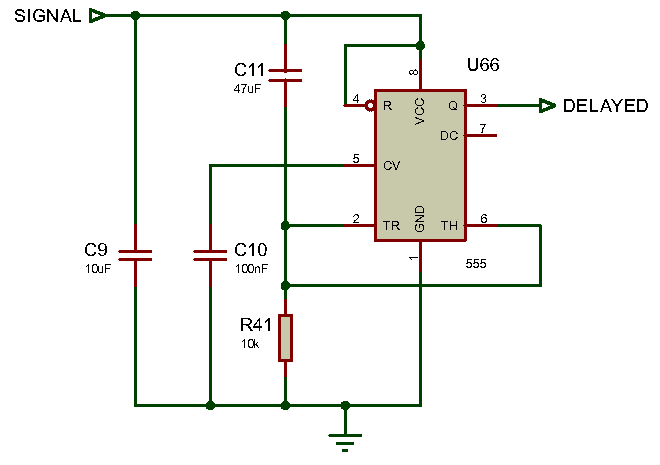
\includegraphics[scale = 1]{Graphics/DELAY/DELAY_STEADY.PDF}
    \caption{Delayed steady ON after a PGT}
    \label{fig:DELAY_STEADY}
\end{figure}

How this circuit works is through the RC network. The combination of the resistor and capacitor forms the RC network. This network determines the length of time it takes to charge the capacitor, i.e. the bigger the resistor and capacitor value, the longer the delay.\medskip

The reason why the circuit doesn't turn on automatically is because pin 2, the trigger pin, initially when the power turns on, is HIGH. This is because the capacitor hasn't charged up yet. Until the capacitor charges up, this pin is HIGH. Since the trigger pin is active LOW, the output will be off until this pin goes LOW. As the capacitor charges up and gets near the supply voltage it is connected to, the voltage at pin 2 decreases. When the voltage at pin 2 gets below 1/3 of the supply voltage, the pin is now LOW. When it is LOW, this is when the output goes HIGH, effectively delaying the input signal.\medskip

In this circuit, capacitors C9 and C10 are there just to decouple the input signal. They have nothing to do with the timing circuit. \medskip

This subassembly is used only once in our circuit. Its function is to delay the \emph{DONE} signal. The purpose of this is to give the Individual Digit Checking GALs some time to perform their operations before checking if the whole password is correct. This delay is needed to overcome the internal propagation delays of the GALs.\medskip


\subsubsection{Delayed impulse after a PGT}
\label{sec:DELAYED_PULSE}

This second circuit is very similar to the first one, the only difference being that instead of a steady ON after a PGT, it only outputs a short pulse after a delay. To achieve this behaviour two 555s have been connected to one another. The first one is connected in the same configuration that we described earlier, that is, it outputs a delayed steady ON after a PGT. The second 555 circuit is a bit more complex. In essence, it behaves as a monostable, as it only outputs a single pulse when triggered. The only difference is that to trigger a monostable, a NGT pulse has to be applied to the Trigger pin (Pin 2), but this cannot be achieved using out configuration as the output of the first 555 is a steady ON. \medskip

\clearpage

To get around this problem, we have used a special tipe of monostable which operation we will describe below.\medskip

\begin{figure}[H]
    \centering
    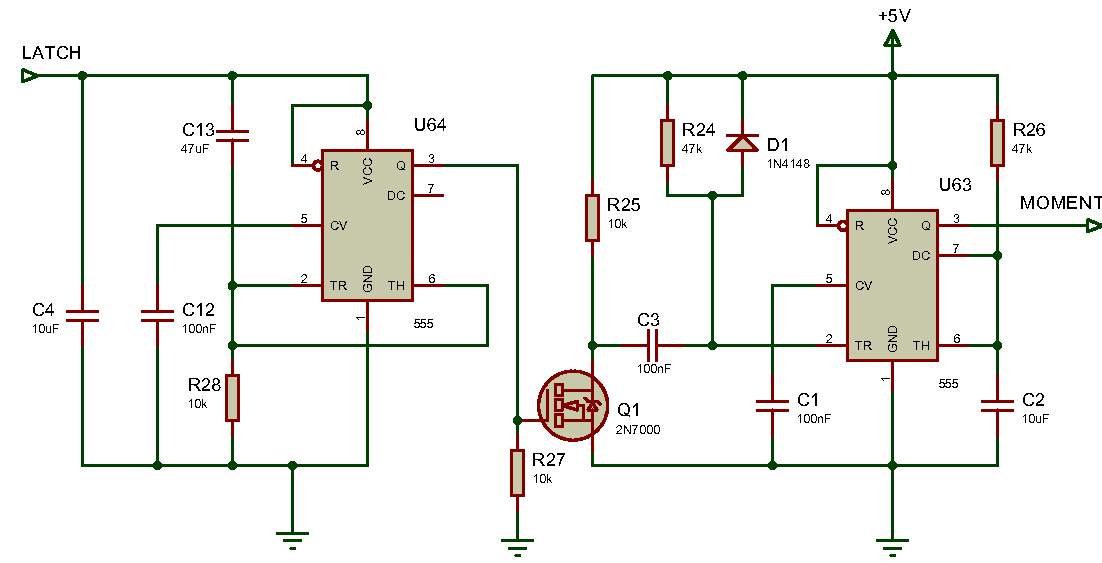
\includegraphics[scale = 0.7]{Graphics/DELAY/DELAY_PULSE.PDF}
    \caption{Delayed impulse after a PGT}
    \label{fig:DELAY_IMPULSE}
\end{figure}


When Q1 is off, that is, when the output of the first monostable is 0V, C3 is in short circuit, meaning that both its leads are at 5V due to the pull-ups R24 and R25, so the voltage drop across it is 0V. The voltage at the Trigger pin (Pin 2) is 5V as well, which means that the output Q (Pin 3) is off, as we need a voltage equal or lower than $V_{cc}/3$ at the Trigger pin to turn it on.\medskip

Once the N-Channel Mosfet is turned on by the first 555, the capacitor is grounded and an RC network is formed by R24 and C3. The voltage in the capacitor is 0V initially, so the voltage in the Trigger pin is 0V as well, turning the output on. As soon as C3 charges, The voltage at the trigger returns to 5V again and the output is switched off. In essence, this simulates the press of a button. \medskip

Q1 is an arbitrary N-Channel Mosfet and R27 is there to discharge its internal capacitor. \medskip

In our circuit, we have used this circuit three times to accomplish various duties such as:

\begin{itemize}
    \item Auto starting the system. (See \textbf{Subsubsection \ref{sec:AUTOSTART}})
    \item Resetting the system once the execution of the code is finished. (\textbf{See Subsection \ref{sec:GENERAL_RESET}})
    \item To wait a few ms before showing the Open/Error message during which the introduced number is shown. (\textbf{See Subsections \ref{sec:PASS_CHECK} and \ref{sec:OPEN_ERROR}})
\end{itemize}
\subsection{General reset}
\label{sec:GENERAL_RESET}

Once the \textbf{\textit{Open}}/\textbf{\textit{Error}} message has been displayed for a few ms, all programmable logic devices must be reset.
\medskip

In order to do this, the \emph{RESET} signal that commands all the GALs, is operated with \emph{ENDPULSE\_SEND} output. This signal can come from two GALs, the \emph{OPEN} and the \emph{ERROR} one, and it indicates when the cycle is over, i.e. when the Open/Error message has been displayed for a few ms and the status LED has either turned red or green. To save some money and space, both of these signals have been connected to an OR gate which output is fed directly into one of the timers mentioned in \textbf{Subsubsection \ref{sec:DELAYED_PULSE}}. The timer's output is connected to the \emph{RESET}, which resets all the state machines.

\begin{figure}[H]
    \centering
    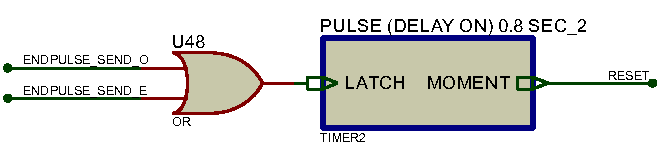
\includegraphics[scale = 1]{Graphics/GENERAL RESET/GENERAL_RESET.PDF}
    \caption{General Reset Proteus Subassembly}
    \label{fig:GENERAL_RESET}
\end{figure}{}
\subsection{Enable Selector \& Autostart}
\label{sec:ENABLE_AUTOSTART}

\subsubsection{Enable Selector}
\label{sec:ENABLE_SEL}

Taking into account the fact that the 4-digit 7-segment displays receive data from different GALs throughout the different stages of the system, short-circuiting the data lines is very easy. We must therefore prevent this from happening so as to have a functioning system.\medskip

To solve this nuisance, an auxiliary GAL is needed. This device will command the \textit{ENABLE} pins of out custom-designed drivers (See \textbf{Subsubsections \ref{sec:DISPLAY}} \textbf{and} \textbf{\ref{sec:OPEN_MESSAGE}} for more information on this topic). This, in essence avoids short circuits by only having one display driver active at the time (The rest being in High-Z mode).

\medskip

The subsystem has the following inputs: the clock signal (\textit{CLK}), the display signal (\textit{DISP\_EN\_}), which comes from the OPEN/ERROR GALs, and the \textit{READY} signal for the autostart. \medskip

On the other hand, the outputs are: \textit{START}, which commands the beginning of the auto start, and the \textit{DISP\_EN} array that regulates the enable signals of the different sub-circuits.\medskip

As \textit{DISP\_EN\_0} corresponds to the \textbf{\textit{Open}} message, each time that it gets pulled HIGH, the \textit{DISP\_EN1}, which corresponds to the OPEN subcircuit enable signal, must be pulled HIGH too.\medskip

The same principle applies to \textit{DISP\_EN\_1}. This signal corresponds to the \textbf{\textit{Err}} message, so each time that it is pulled HIGH, the \textit{DISP\_EN2}, which corresponds to the ERROR subcircuit enable signal, must be pulled HIGH too.

\medskip

When none of these input signals, i.e. \textit{DISP\_EN\_0} and \textit{DISP\_EN\_1} are HIGH, that means that the display does not have to show neither the \textbf{\textit{Open}} nor the \textbf{\textit{Err}} message, but the password entered by the user. Thus, \textit{DISP\_EN0}, which is the enable for the decoder of the password, must be pulled HIGH.\medskip

\subsubsection{Autostart}
\label{sec:AUTOSTART}

The autostart subsystem, as the name suggests, is in charge of starting the system automatically when the simulation begins. This is needed because the ring counter that we discussed in \textbf{Subsection \ref{sec:KEYPAD}} needs to be pre-loaded in order to start.\medskip

In a real case scenario, a single pulse generator, such a monostable could be used to generate the required pulse. For the simulation though, it is a tad more complex, as the simulation takes some time to load, and non-linear components such as diodes tend to act in a weird way if they are powered before starting it. That is why we cannot simply connect one of the pulse generators that we discussed in \textbf{Section \ref{sec:DELAYED_PULSE}} to the \textit{START} signal and expect it to run flawlessly. \medskip 

\clearpage

To overcome this problem, we have simply delayed the operation of the pulse generator by performing some unnecessary actions. Since we had some pins left in the Enable Selector GAL, we decided to use it to generate said delay. In the code we can see that the GAL reads the value of the \textit{READY} signal, which is HIGH when the simulation starts and it checks that it is indeed HIGH, and as a consequence, it pulls the \textit{TURN\_ON} HIGH. After that, the signal passes through a buffer, so as to add its propagation time to the one of the GAL, and, finally, the pulse generator is triggered, pre-loading the initial ring counter and starting the system.\medskip

This part of the code would not be needed in a real case scenario as its only function is to wait for the simulation to load properly before starting the system. \medskip

The VHDL code that describes this subsystem can be found below:

\inputcode{Code/ENABLES.vhd}

The Proteus Subassembly of both circuits is attached below:

\vspace{-0.5cm}

\begin{figure}[H]
    \centering
    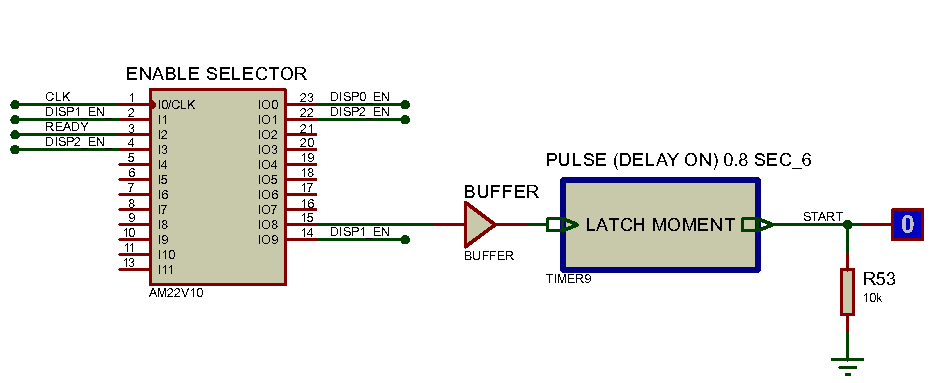
\includegraphics[scale = 0.85]{Graphics/ENABLE SELECTOR + AUTOSTART/ENABLE_SELECTOR_AUTOSTART_PROTEUS.PDF}
    \caption{Enable Selector \& Autostart Proteus Subassembly}
    \label{fig:my_label}
\end{figure}{}

\section{Conclusion}

In a nutshell, this project has posed an interesting challenge and it has given us the oportunity to not only learn about VHDL in the process but also to work with the different modules and ICs that we have seen in the course.\medskip

Out system is able to perform the duties that we initially intended it to perform even after taking into account the limitations of the hardware that we have used. The restrictions of the GAL PLDs in terms of input/output ports, memory capacity and the programming language, which was new to us in a sense, have made us use a considerable number of GALs, which only proves how far technology has come in the past few years. This project could have been implemented more easily using CPLDs or even FPGAs or, in the other side of the spectrum, a simple microcontroller. \medskip

Even though we have managed to create a fully functional safe deposit box, there are lots of things to improve nonetheless:

\begin{itemize}
    \item Passwords can only have 4 digits, and the same number cannot be repeated consecutively.
    
    \item To introduce and validate a password one must press \textit{*} and \textit{\#} , which makes the process slower.
    
    \item The code is most probably not as efficient as it could be. Improving it would eliminate some PLDs making the device not only more compact but also cheaper and easier to implement.
    
    \item The set password mechanism requires the user to know the binary code of the password, which is something a bit inconvenient.
    
    \item As we have said before, the use of CPLDs, FPGAs, or microcontrollers would greatly help reduce the size of the project.
\end{itemize}


All in all, we think that this project has served not only to wrap up the knowledge that we have acquired in this subject but also to learn to work as a team, mostly due to the complexity of certain parts. We sincerely hope you enjoy it as much as we have enjoyed putting it together. 

\clearpage
\printbibliography


\end{document}